% This example An LaTeX document showing how to use the l3proj class to
% write your report. Use pdflatex and bibtex to process the file, creating 
% a PDF file as output (there is no need to use dvips when using pdflatex).

% Modified 

\documentclass{l3proj}
\begin{document}
\title{Team V - How Not To Kill Your Dog}
\author{Ross Adam \\
        Andrew Gardner \\
        Nicole Kearns \\
        Mamas Nicolaou \\
        Asset Sarsengaliyev}
\date{18 March 2013}
\maketitle
\begin{abstract}

This project aims to produce a learning application to be used within the University of Glasgow School of Veterinary Medicine by students wishing to revise and test their knowledge.  The Django Web Framework was used to produce a web based application that is hosted in the veterinary school. It consists of both teaching slides with course content and affiliated questions. There is also administration functionality to allow the course co-ordinator to edit the content of the application to evolve with the prescribed course content.

\end{abstract}
\educationalconsent
\tableofcontents

\chapter{Introduction}
\label{intro}



\section{Motivation}
Team V is comprised of five students currently in their third year of a Computing Science degree at the University of Glasgow. The team will be working for 7 months on this project which is the sole piece of coursework for the Team Project 3 course. By the end of this period of time it is hoped that there will be a fully functional piece of software that can be delivered to our client.
\newline
\newline
This project is ``How not to kill your dog'' a macabre title for our veterinary student revision program. Our client is Dr Fiona Dowell, a senior lecturer at the University of Glasgow's Veterinary School. In addition to our client there are several more stakeholders for this application: the veterinary students who will be using this application throughout their studies; other lecturers and finally I.T. support staff who will interact with this application extensively.  Dr Dowell found that her students struggle with learning how to do drug calculations more than they do with any other part of their course. She came up with the idea of having an application available to veterinary students to help enhance their drug calculation skills.
\newline
\newline
Dr Dowell believes that students will find it more entertaining to have a game-like learning application, which they could use in their free time to entertain themselves, but also learn and become better with their drug calculations. She would therefore like a program that can be used as a revision aid for students which she can add her own educational slides to and create tests and questions to engage students.
\newline
\newline
The motivation for developing this software was to bring all the education resources currently in use and create a more centralised location. Currently the client simply uses PowerPoint slides filled with information which her students can download from their respective Moodle site. Using our software would allow the user to forgo the need for specific software to read .ppt extension files and reduce compatibility issues. Also users do a lot of calculations and all tests with pen and paper; with new software it would be hoped that calculations could be performed online which would automatically compare them and tests would be submitted online for marking. This would result in faster and more efficient work for both students and lecturers. Dr Dowell also considered the possibility of promoting this application outside of the the veterinary school in hopes of further enhancing the reputation of the University of Glasgow.

\section{Project Aim}

The aim of the project was to create a learning application for veterinary students that allows them to learn new content and revise and refresh existing knowledge. As this project has been heavily client dependant the team has had several meetings with Dr Dowell to ensure that high quality software that meets her requirements has been produced.
\newline

Through this process we have identified these aims for the project:
\newline

\begin{itemize}
\item To centralise existing revision material.
\item Provide a system students can use to learn and revise course content.
\item Provide a system which can include informal test material to assure students of their knowledge.
\item Allow the evolution of the application content to match course content through the adding, deleting and editing of topic slides and questions.
\item Make the learning process engaging and enjoyable for users.
\end{itemize}   

\section{Dissertation Outline}

The dissertation outlines in detail the process of carrying out the ``How Not To Kill Your Dog'' project. Below is an outline of our report:

Chapter 2 discusses existing applications and similar revision tools which we found useful in the design process.

Chapter (Requirements) discusses the requirements gathering process and outlines the functional and non-functional requirements for our application.

Chapter (Design) discusses the general design of the application.

Chapter (Implementation) discusses the implementation of the project.

Chapter (Testing)

Chapter (Evaluation)
\chapter{Background}
\label{background}

This section discusses several different existing artifacts, both medical applications and other revision tools. These applications were selected to provide inspiration for our own application design, specifically assessing the current tools within the market and how each displays their content to the user.

\section{Investigation of Existing Artifacts}


There are a few similar tools and learning resources available for vetinary students. This section discusses some of the current tools and a few tools which our client, Dr Fiona Dowell, has shown us in order to give us an idea of what she wanted for the application.

\subsection{Medical Helper Applications}


\subsubsection{NHS Adult Drug Calculations}

\begin{figure}[!htb]
\minipage{0.32\textwidth}
  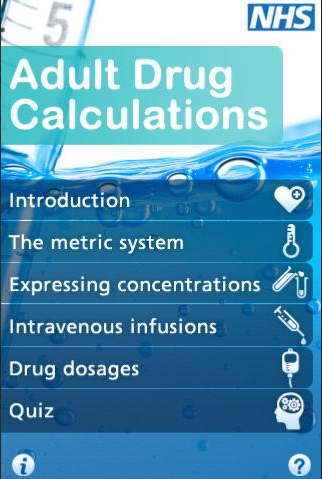
\includegraphics[width=\linewidth]{images/NHSDrugApp/NHSDrugApp2.png}
\endminipage\hfill
\minipage{0.32\textwidth}
  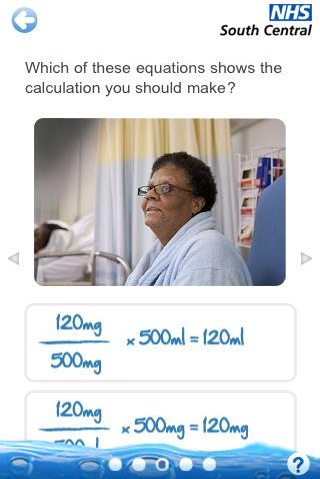
\includegraphics[width=\linewidth]{images/NHSDrugApp/NHSDrugApp4.png}
\endminipage
\end{figure}


The NHS Adult Drug Calculations is a smartphone based learning tool aimed at nurses and midwives who are newly qualified or returning to practice. The tool allows the user to browse through different topics. Within each topic, there are a number of slides providing the user with the information and theory behind the calculations, and then has a few ``Check your knowledge'' slides containing multiple choice questions to test the user on what they have read. The interface is very simple and easy to use. The main menu allows the user to simply select which topic they qish to go over. Within each topic, there are arrows on each page which will allow the user to navigate back and forward between the pages and there are breadcrumbs at the bottom of each page indicating how far through the topic they are.  There is also an arrow at the top left-hand corner which will allow the user to return to the main menu at any point. One feature which is particularly useful to new users is the help button, which informs the user how to use the application. This application is very similar to the application which our client would like for the vetinary students.

\subsubsection{Vet Calculator}

\begin{figure}[!htb]
\minipage{0.32\textwidth}
  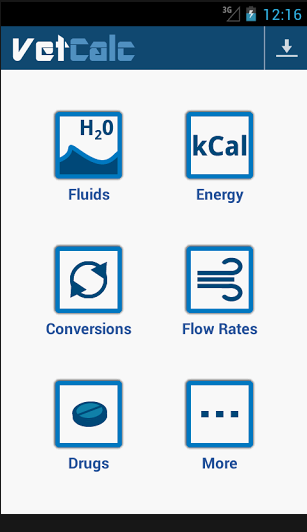
\includegraphics[width=\linewidth]{images/VetCalcApp/VetCalcApp1.png}
\endminipage\hfill
\minipage{0.32\textwidth}
  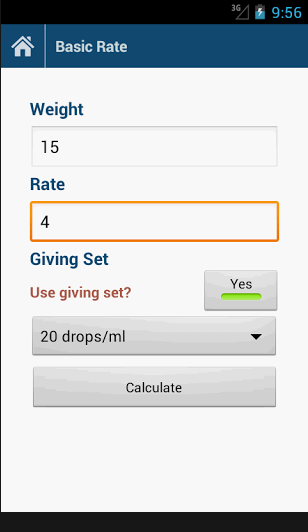
\includegraphics[width=\linewidth]{images/VetCalcApp/VetCalcApp3.png}
\endminipage\hfill
\minipage{0.32\textwidth}%
  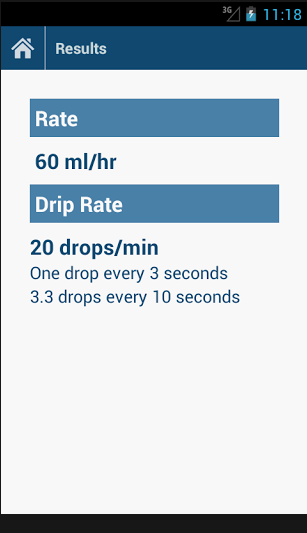
\includegraphics[width=\linewidth]{images/VetCalcApp/VetCalcApp4.png}
\endminipage
\end{figure}

VetCalc is an android based tool aimed at verterinarians, students, nurses and technicians, which allows the user to enter the necessary details, such as weight; dose; formulation; volume of fluid; etc. and will produce the result for the user. The interface for the vet calculator is very simple and easy to use. The menu is a simple grid-layout of different topics and sections for drug calculations. Within each topic, the user has to simply enter the necessary details into the clearly labelled text boxes and click 'Calculate' in order to get the result of the calcuation. On each page, there is a home button which will easily allow the user to return to the main menu at any point. This application is useful for users who simply need to get the results of a calculation. However, out client wants an application that will teach the students how to carry out the calculations and not simply produce the result for them as they will need to know how to carry out these calculations throughout their career.

\subsection{Revision Tools}

Before desgining our own application the team agreed that we should
research existing tools for revision. The following were suggested as
members had had some experience using them. 

\subsubsection{Bitesize}
The Bitesize revision tool is a service provided by the BBC which
operates in the user's web browser. It is a simple implementation of
linked webpages that cover a variety of subjects from across the UK
national curriculum. The team chose to research the Bitesize system
because several of the Scottish Students had used it before and found
it helpful for their studies at high school. First we decided to analyse how the
content is displayed within the tool.\\

\begin{figure}[!htb]
\caption{Bitesize Layout}
 \centering
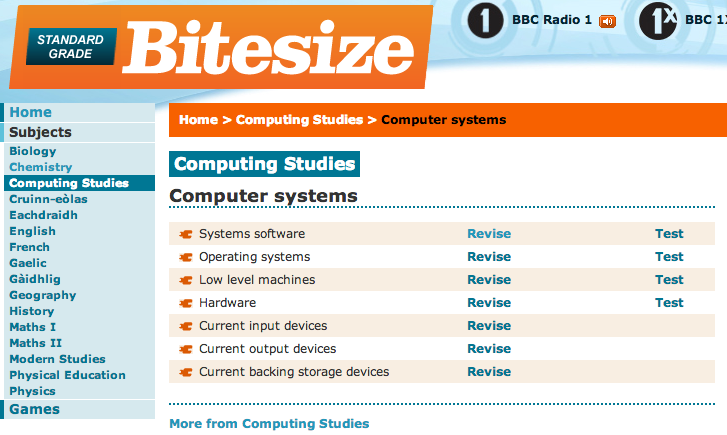
\includegraphics[width=0.9\textwidth]{images/Bitesize/BitesizeLayout.png}
\end{figure}

Figure 1.1 shows the typical layout of a Bitesize page: each page of
content is framed by the Bitesize logo (implemented as a clickable image that
returns the user to the main page) and on the right of the screen is
the index for various subjects allowing for quick navigation.\\

\begin{figure}[!ht]
\caption{Bitesize Content}
 \centering
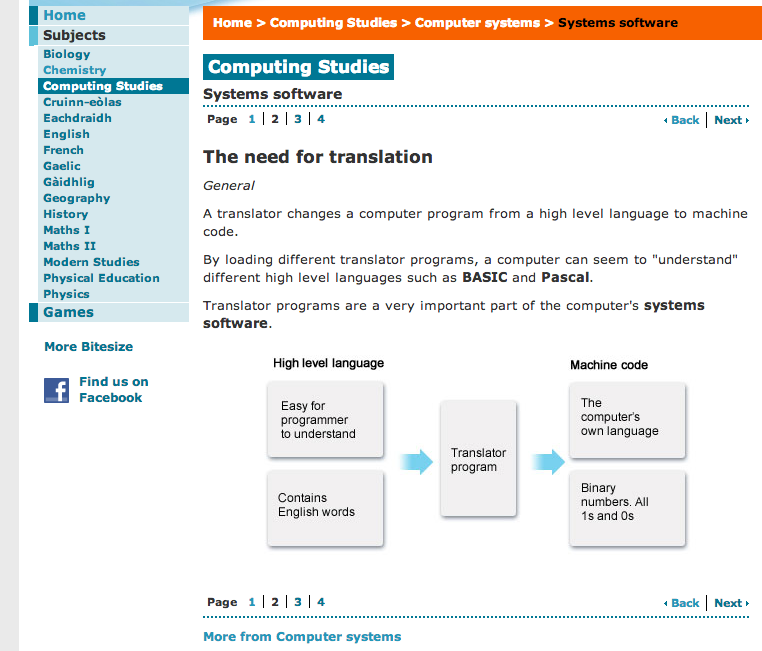
\includegraphics[width=0.9\textwidth]{images/Bitesize/BitesizeContent.png}
\end{figure}

A consistent frame is a concept that Team V also wanted to achieve
within our own design. Instead of a bitesize logo we would use the
Veterinary School logo which would make our application appear more
professional. Our index page will feature links to different topics
for fast navigation for experienced users.\\


Figure 1.2 illustrates how each page is displayed in the tool. Content
is simply loaded into the page in the center and navigation is
achieved by clicking specific buttons. Our goal is to have a simple
slider to sequentially navigate pages.\\
\newpage
\subsubsection{Hot Potatoes}

The second system Team V assessed was Hot Potatoes, a simple quiz
creation system that allows users to create online quizzes which they
can then publish for other users to interact with.\\ 

\begin{figure}[!htb]
\caption{Hot Potatoes Program}
 \centering
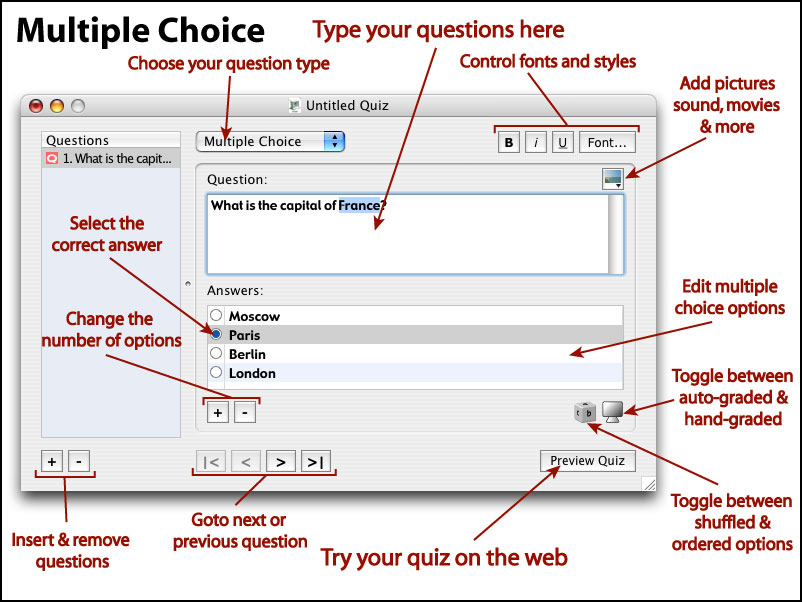
\includegraphics[width=0.9\textwidth]{images/HotPotatoes/HotPotatoesQuestion.jpg}
\end{figure}

The system itself is a comprehensive suite of features and programs
that can produce different types of quizzes: multiple choice; image
matching and several more.\\

The included figure shows how a user can create a multiple choice question. This is much more complex than our implementation will be but it gave us an idea of how to make the process streamlined and easier for the user to work with.\\ 

The client has requested a system that includes questions which can be
answered at the same time as the course content is being
displayed. This would hopefully ensure the student retained the
information better than simply reading the slides. Our system will
only allow multiple choice questions to be created.

\chapter{Requirements}
\label{req}

This section discusses the requirements elicitation process for our project. As we have an external-client, this process is important to ensure that we identify all requirements to produce the application that fully meets their needs.

\section{Client Interview}

The project was proposed by Dr Fiona Dowell, a senior lecturer at the University of Glasgow School of Veterinary Medicine. Initially, we met with Dr Fiona Dowell in order to gain more information about the requirements and specification for the application to ensure that we produced an application relevant to what the client wanted.\\

Our initial requirements for the vet application were:

\begin{itemize}
\item A learning application for vet students, providing step-by-step tutorials for different sections of the vet course.
\item Simple example questions within each topic to test how much the user is learning about that specific section.
\item A larger assessment at the end of all sections to test users on all the content within the application.
\end{itemize}

After the initial meeting with our client, we thought that it would be useful for the content within the application to be able to be updated , for example if the content changed; to fix errors or update to include different questions. We presented this idea to the client who agreed that this would be a useful feature as it might be good to be able to update after some user feedback. The functional requirements were then updated to include an administration system.\\
The administration system allows admin staff to upload and remove topics. It also allows the content of each topic to be updated, slides and questions can be added and removed.


\section{Functional Requirements}

\subsection{Requirements Table}

\textbf{Student -} Uses the application to browse through the different topics, answering the topic-related questions as they go along and completing the final assessment at the end.

\textbf{User Admin -} Responsible for adding new users to the system, setting their permissions to determine their access levels and deleting them when necessay.

\textbf{Content Admin -} Responsible for adding new topics, slides and questions to the system, and ensuring that all content is kept up to date with the course content.

\textbf{Student}\\

\begin{center}
\begin{tabular}{|c|c|}
\hline \textbf{Id} & \textbf{Requirement}\\
\hline SR1 & View Topic\\
\hline SR2 & View Slides\\
\hline SR3 & View Questions\\
\hline SR4 & Answer Questions\\
\hline 
\end{tabular}
\end{center}

\textbf{User Admin}\\

\begin{center}
\begin{tabular}{|c|c|}
\hline \textbf{Id} & \textbf{Requirement}\\
\hline UAR1 & Add User\\
\hline UAR2 & Delete User\\
\hline UAR3 & Set Permissions\\
\hline 
\end{tabular}
\end{center}

\textbf{Content Admin}\\

\begin{center}
\begin{tabular}{|c|c|}
\hline \textbf{Id} & \textbf{Requirement}\\
\hline CAR1 & Add Topic\\
\hline CAR2 & Edit Topic\\
\hline CAR3 & Delete Topic\\
\hline CAR4 & Add Slide\\
\hline CAR5 & Delete Slide\\
\hline CAR6 & Add Questions\\
\hline CAR7 & Edit Questions\\
\hline CAR8 & Delete Questions\\
\hline 
\end{tabular}
\end{center}


\subsection{Use Case Diagrams}

\begin{center}
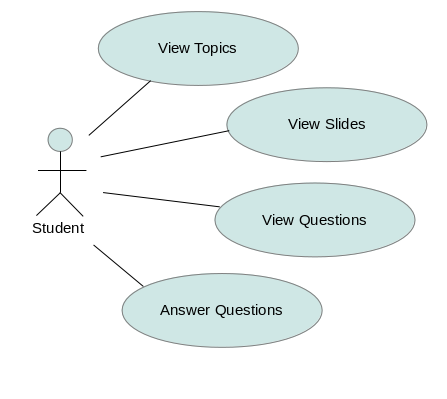
\includegraphics
[scale=0.5]
{images/Student.png}
\end{center}
\begin{center} Student \end{center}

\begin{center}
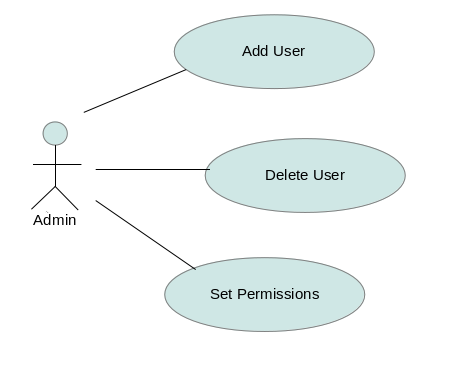
\includegraphics
[scale=0.5]
{images/UserAdmin.png}
\end{center}
\begin{center} User Admin \end{center}

\begin{center}
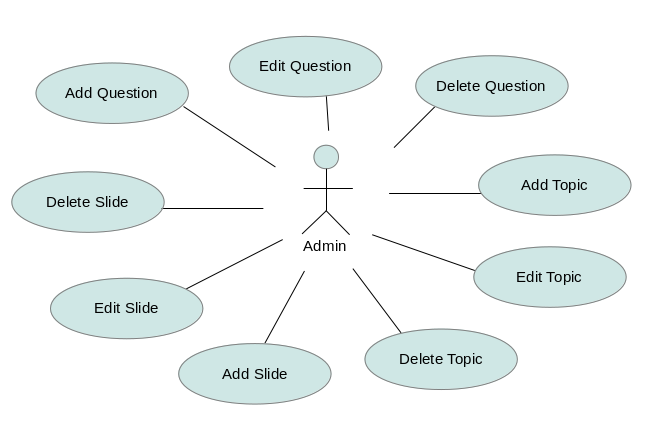
\includegraphics
[scale=0.5]
{images/ContentAdmin.png}
\end{center}
\begin{center} Content Admin \end{center}

\subsection{Student Requirement Details}

\textbf{SR1: View Topics}\\
\textbf{Description}: Users must be able to view the different topics in the application. \\
\textbf{Rationale}: The students must be able to view the different topics in the application. This will allow them to navigate through the different topics as the progress through the slides and topics.\\
\textbf{Priority}: Must Have \\


\textbf{SR2: View Slides}\\
\textbf{Description}: Users must be able to view the different slides in the application. \\
\textbf{Rationale}: The students must be able to view the different slides in the learning application. The student will be able to navigate back and forward through the different slides of a topic and read through the content on each page.  \\
\textbf{Priority}: Must Have\\


\textbf{SR3: View Questions}\\
\textbf{Description}: Users must be able to view the different questions in the application. \\
\textbf{Rationale}: The student must be able to view the questions in the application. This will allow the students to go through the different questions related to the information given in the slides.\\
\textbf{Priority}: Must Have\\


\textbf{SR4: Answer Questions}\\
\textbf{Description}: Users must be able to answer the questions in the application.\\
\textbf{Rationale}: The student must be able to answer the questions in the learning application. This will allow the students to test the knowledge they learned from the information provided in the slides. \\
\textbf{Priority}: Must Have\\
\textbf{Dependencies}: SR3\\


\subsection{User Admin Requirements Details}

\textbf{UAR1: Add User} \\
\textbf{Description}: The admin user must be able to add a user.  \\
\textbf{Rationale}: The admin users must be able to create a new user account to allow other users to use the application and have access to the content management.\\
\textbf{Priority}: Must have \\

\textbf{UAR2: Delete User} \\
\textbf{Description}: The admin user should be able to delete a user. \\ 
\textbf{Rationale}: The admin user should be able to remove users from the system, meaning that they will no longer be able to login or have access to any of the content management.\\
\textbf{Priority}: Should have \\
\textbf{Dependencies}: UAR1\\

\textbf{UAR3: Set Permission} \\
\textbf{Description}: The admin user must be able to set user permissions.\\
\textbf{Rationale}: The admin user must be able to set user permissions in order to provide users with the appropriate access.\\
\textbf{Priority}: Must have \\
\textbf{Dependencies}: UAR1\\

\subsection{Content Admin Requirements Details}

\textbf{CAR1: Add Topic}\\
\textbf{Description}:  The admin users must be able to add a new topic. \\
\textbf{Rationale}: The admin user must be able to create a new topic within the admin site. \\
\textbf{Priority}: Must have\\


\textbf{CAR2: Edit Topic}\\
\textbf{Description}: The admin users should be able to edit a current topic.\\
\textbf{Rationale}: The admin user should be able to edit a current topic for the application. This will allow the admin user to update the topic if it any details change or are inaccurate.\\
\textbf{Priority}: Should Have \\
\textbf{Dependencies}: CAR1\\

\textbf{CAR3: Delete Topic}\\
\textbf{Description}: The admin users must be able to delete a current topic. \\
\textbf{Rationale}: The admin users must be able to remove a current topic from the application. This will mean that the topic will no longer be available within the application.\\
\textbf{Priority}: Must Have \\
\textbf{Dependencies}: CAR1\\

\textbf{CAR4: Add Slide}\\
\textbf{Description}:  The admin users must be able to add a new slide. \\
\textbf{Rationale}: The admin users must be able to add new slides to the application. This will provide the content for the students to browse through. \\
\textbf{Priority}: Must Have\\

\textbf{CA56: Delete Slide}\\
\textbf{Description}: The admin users must be able to delete a slide.\\ 
\textbf{Rationale}: The admin users must be able to remove a slide from the application. This means that selected slide will no longer be available in the application.\\
\textbf{Priority}: Must have\\
\textbf{Dependencies}: CAR4\\

\textbf{CAR6: Add Question}\\
\textbf{Description}: The admin users must be able to add questions to the application. \\
\textbf{Rationale}: The admin users must be able to create new questions and add them to the application, allowing the students to test how much they have learned.\\
\textbf{Priority}: Must Have\\

\textbf{CAR7: Edit Question}\\
\textbf{Description}: The admin users should be able to edit questions.\\
\textbf{Rationale}: The admin users should be able to edit questions. The users should be able to update the questions to keep the questions up to date or to fix error.\\
\textbf{Priority}: Should Have \\
\textbf{Dependencies}: CAR6\\

\textbf{CAR8: Delete Question}\\
\textbf{Description}: The admin user must be able to delete questions. \\
\textbf{Rationale}:  The admin user must be able to remove questions from the application. This will mean that the question is no longer available on the application for the students to view.\\
\textbf{Priority}: Must have\\
\textbf{Dependencies}: CAR6\\

\section{Non-Functional Requirements}

\begin{center}
\begin{tabular}{|c|c|}
\hline \textbf{ID} & \textbf{Non-functional Requirement}\\
\hline NFR1 & Availability\\
\hline NFR2 & Performance\\
\hline NFR3 & Educational\\
\hline NFR4 & Portability\\
\hline NFR5 & Concurrency\\
\hline
\end{tabular}
\end{center}

\textbf{ NFR1: Availability}\\
As our application is a web-based application, it is important that users are able to access the application at all times, provided that the server it is running on is operational.

\textbf{NFR2: Performance}\\
Performance is an important part of the usability of our application. Our application should be able to load content from the database and display it within our application in a short amount of time. Failure to do so may result in the application being an inefficient and ineffective learning tool.\\

\textbf{ NFR3: Educational}\\
The application should be educational to users, whether it be new information or revising the material. Allowing the users to read through the slides and answer related questions should enhance the user's knowledge.

\textbf{ NFR4 : Portability}\\
Having a web-based application means that our application is not restricted to a certain operating platform. This means that our application should be able to run on any platform without having to install additional software.

\textbf{ NFR5: Concurrency}\\
As a study tool we know that many users will be accessing the software simultaneously when there are upcoming exams and tests. The application must therefore support concurrent user access to the system.

\chapter{Design}
\label{design}

This chapter covers the various aspects of the application's design process. As our project was client-based the design was very much focused on satisfying the requirements laid out in the previous chapter. Fiona Dowell, our client from Glasgow University's Veterinary School, evaluated our initial user interface design and we then revised it according to the feedback that we received from her. When we were satisfied with the design we moved on to the implementation phase.

\section{Design Goals and Considerations}

The overall design goals for the application follow principles already well established in the field of web development.

These were:

\begin{enumerate} 
\item{\textbf{Precedence}} \\
The use of positioning, colour, size and contrast to naturally guide the user around the application. For example, most sites have a logo featured in the top left corner because studies have shown this to be the first place users look when accessing web sites. This enables natural navigation sequences: elements like the navigation bar being strategically placed so users' eyes will follow from the larger, relatively contrasted logo to the navigation bar.

\item{\textbf{Navigation}} \\
The principle of making it easy and intuitive for users to navigate your web site. For example, links and buttons should be well positioned and clearly indicate their function while offering appropriate feedback when clicked. Measures should also be taken to inform the user where they are currently within the application.

\item{\textbf{Typography}} \\
The text of a web application is the most common element of design and therefore deserves significant consideration. Font type, size, spacing and colour are essential to the application's overall clarity and readability.

\item{\textbf{Usability}} \\
The encompassment of previously defined principles such as precedence, navigability and text. They relate to how usable the application is for its users. An important usability consideration is that of 'standards adherence'. This is the following of conventions laid out and used by millions of other websites, such as underlined text indicating a link.

\item{\textbf{Consistency}} \\
The principle of making the application's design elements ``match'' coherently between pages and on the same page of the site. Attributes like colour and font choice, for example, should remain consistent across the site.

\item{\textbf{Clarity}} \\
The appropriate use of design techniques such as positioning, contrast, font aliasing and others to make your design stand out crisply and clear. 
\end{enumerate}
	
\subsection{Admin}

The admin user is solely responsible for the content management of the application. With that in mind we approached the admin interface's design with a heavy focus on usability and navigation, rather than fancy themes and textual styles. We felt that the admin interface should possess a natural gravitas; that it should be taken seriously as a tool that controls the entire functionality of the application and not as a novel feature. To this extent our goal was to use a very simple theme, contrasting sharply in style and presentation with the student user interface. This was a wilful breaking of the consistency design principle to enforce a measure of aforementioned seriousness onto the admin interface.

We also had to consider that the likely admins of the application would be relatively inexperienced with regards to administrating an entire web application's content. Being mindful of this we had to design the interface to be accommodating for the inexperienced, allowing for easy navigation and informative feedback with every action taken.

\subsection{Student}

In stark contrast to that of the admin user interface, the student's view of the web application had to embody all design goals previously defined in this chapter. They had to be able to navigate the site easily, knowing where they were at all times and how to get to where they would like to go with no fuss or ambiguity.

As this application's core functionality is assessment based it was important to have a gentle colour theme that would contrast naturally with the displayed content and not distract the user. This also held true with appropriate user feedback. We made an early design decision to provide the user with timely responsive feedback when answering questions.

An important design goal was to create an interactive learning experience for the user. In order to achieve this we decided to include an animal avatar with an associated health bar. A correct answer would have no effect whereas an incorrect answer would result in health loss. This design feature helps to engage the student on a personal level as their progress will affect the animal's lifespan. 

\section{Initial Design}

\subsection{ER Diagram}
	
After establishing our initial design goals we created an entity relationship diagram. Defining our data models at this phase allowed us to clearly understand the distinction between entities and how they relate to each other.

\begin{figure}[!htb]
\caption{Application ER Diagram}
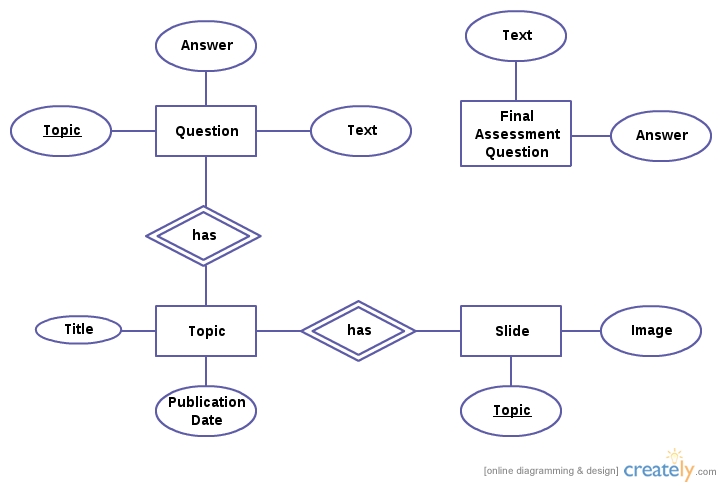
\includegraphics[width=\linewidth]{images/ERDiagram.png}
\end{figure}

\subsection{Paper Prototypes}

Paper prototyping was an effective and inexpensive method used to determine the design direction of the student user interface. The use of paper prototypes allowed us to experiment with various design configurations without the overhead of time and resources. This method of design was particularly suited to this application as it was simple to review and to iterate upon. Client involvement was a requirement for the success of the project. Therefore it was imperative that our early design ideas were subject to client review and feedback. Sending several prototypes for client evaluation meant that there was more potential for varied, constructive feedback. Receiving said feedback from the client afforded us more opportunity to revise our designs in accordance with their wishes. 

The paper prototypes aimed to fulfil the student user's functional requirements as laid out in the previous chapter. This meant that we had to design mechanisms for the following use cases:

\begin{itemize}
\item{Viewing Topics\textbf{ (SR1)}}
\item{Viewing Slides\textbf{ (SR2)}}
\item{Viewing Questions\textbf{ (SR3)}}
\item{Answering Questions\textbf{ (SR4)}}
\end{itemize}

As will be discussed in the Prototype Evaluation section, our client indicated that two prototypes were particularly suitable in meeting the requirements of the application.

\begin{figure}[!htb]
\caption{Topic View}
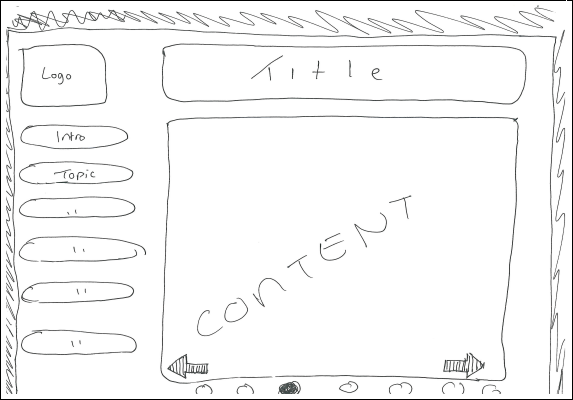
\includegraphics[width=\linewidth]{images/Prototype2.png}
\end{figure}

\begin{figure}[!htb]  
\caption{Final Assessment}
 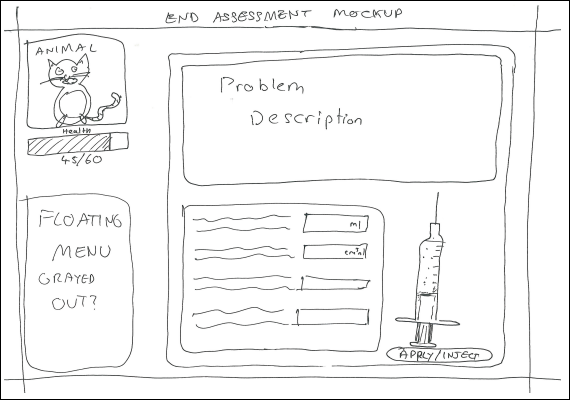
\includegraphics[width=\linewidth]{images/Prototype1.png}
\end{figure}

Figure 4.2 shows the individual topic view for the student user interface. The ``title'' at the top of the page represents the topic's name, with the slides for the topic being shown in the ``content'' section. The arrows contained within the content section represents the possibility of a slider being used, enabling the user to easily switch back and forth between slides. The breadcrumbs, shown below the content box, were designed to enhance user navigability by allowing the user to directly select a slide to navigate to. The rounded buttons to the right of the content section represent clickable links to navigate between individual topics. These design elements satisfy requirements \textbf{SR1} and \textbf{SR2}.

This prototype satisfies design goals laid out in the beginning of this chapter. The judicious use of whitespace enhances the user interface's clarity. With regards to design precedence, the size of the content box (compared to other design features) functions as a focal point, demanding the user's attention. 

Figure 4.2 shows the final assessment page for the student user interface. The inclusion of an animal avatar and health bar satisfies the design goal of interactive student engagement, resulting in a heightened learning experience. Similar to Figure 4.3, the use of whitespace and size precedence allows the user to understand and easily navigate the interface presented to them. The problem description section represents the functional requirement \textbf{SR3} and the box below plus the apply/inject button represents the functional requirement \textbf{SR4}.  

We chose not to create a paper prototype of the admin interface because we knew that Django (the web framework we had chosen to implement the application with) would provide a suitable pre-defined interface. This will be discussed further in the Admin User Interface Subsection. 
 
\subsection{Prototype Evaluation}

The evaluation process involved sending the paper prototypes to our client, Fiona Dowell. This was an important part of the design process as her feedback would naturally impact the application's final design. 

With regards to the paper prototypes, the feedback confirmed our initial design choices. Both designs preferred by our team were also chosen by Fiona and her colleagues. The decision to revise and continue with these designs was reinforced by our client's feedback. This not only resulted in an easy design decision but also supported the overall design direction we had previously agreed on. While we knew further iteration and changes were likely required for implementation, we felt this was a solid base to start from.

\section{Interface Design}

This section covers the user interfaces for both admins and students, analysing how the design meets specific functional requirements and overall design goals.

\subsection{Admin User Interface}

\begin{figure}[!htb]
\caption{Admin User Interface}
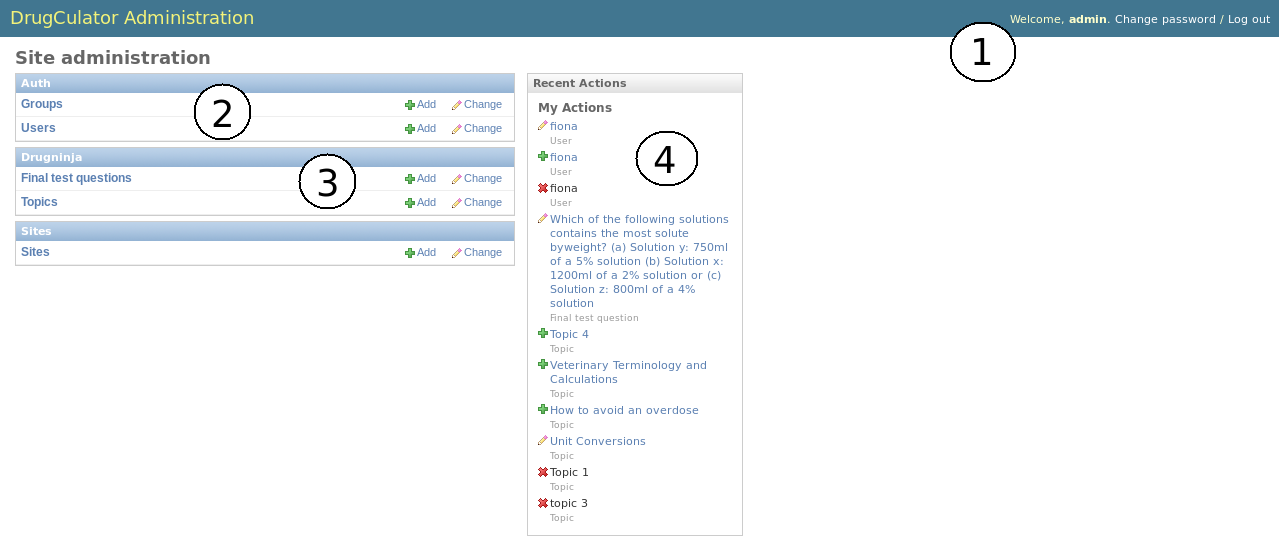
\includegraphics[width=\linewidth]{images/admin_interface1.png}
\end{figure}

Figure (4.4) shows the main page of the admin interface after the admin user has logged in. The interface's specific design theme was largely out of our hands as Django provided this for us. The lack of design control wasn't an issue however, as it conformed to our earlier design goals that the interface should be sufficiently different in theme and style from the student user interface. As figure (4.4) shows, the overall theme is quite minimalistic. There is no extraneous details or features that could distract the admin user.

Annotation 1 shows the welcome message and menu for the user that has just logged into admin interface. It's placement at the top right hand side of the screen adheres to current best practise in web development, which in turn increases the usability of the interface. In terms of typography, the use of bold text confidently directs the user's eye towards expected features such as ``Change password'' and ``Log out''.

Annotation 2 highlights several of the user administration use cases in that they should be able to add, remove and edit current users within the application. These options are displayed logically by being grouped together and have icons that adhere to common user interface idioms. For example the ability to add a user is annotated with a plus symbol, enabling inexperienced users to intuitely deduce how that function would operate. 

Annotation 3 covers the content administrator's functional requirements in being able to add, edit and remove topic content. This annotation's style is identical to that of annotation 2, in that it contributes to the overall consistency of the admin user interface, providing a clear and usable experience for the user. As with annotation 2 a clearly recognisable icon (a pencil) is used to indicate that the link in question leads to editing options for the topics. 

Annotation 4 shows the ``Recent Actions'' bar of the interface. This enables admin users to see all their previous administrative actions for the application. This is very useful as it allows the administrator to track down previous changes to content and navigate to them directly. This navigation is further enhanced by the blue colour of the text, indicating that the text is a link and can be clicked. This blue text link consistency greatly adds to the expected functionality and to the usability of the interface as a whole.

The only design issue we faced with the admin user interface was the lack of creative control over the look and feel. While we still felt it was appropriate and suitably met our design considerations, it would have been better if Django allowed us greater customisation.

\subsection{Student User Interface}

\subsubsection{Main Content Screen}

\begin{figure}[!htb]
\caption{Content Screen}
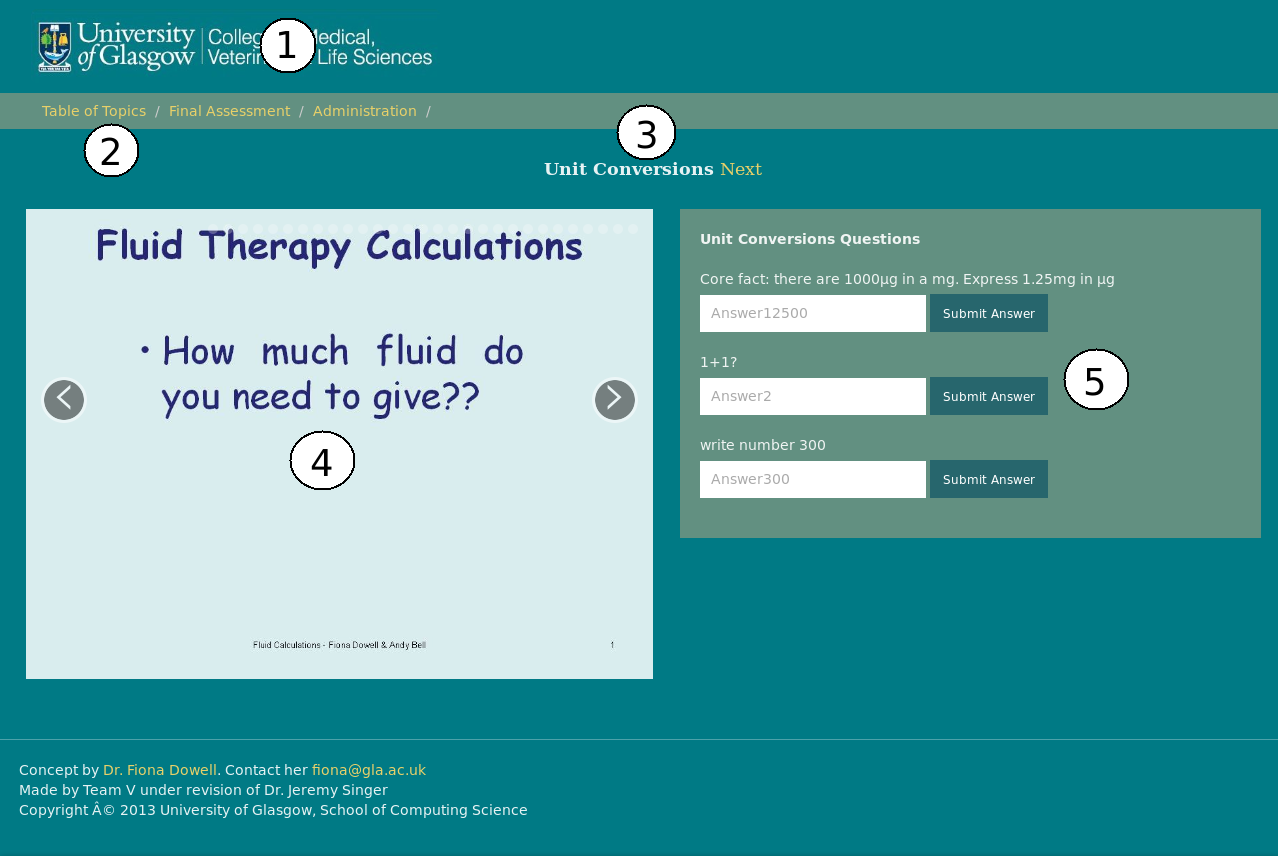
\includegraphics[width=\linewidth]{images/topic_page_annotated.png}
\end{figure}

Figure 4.5 shows the main page users will see when they interact with the system.

Annotation 1 highlights the image of the University of Glasgow's Veterinary School logo. This was included for two reasons: firstly it identifies the University to external bodies that may stumble across the application. Secondly it makes it appear more professional and therefore improves the overall aesthetics.

Annotation 2 shows the application's main navigation section. These are clearly labelled for clarity to identify their purpose. This also has the additional property of increasing usability. Expert users such as students who have used the program before and want to jump to a specific page can utilise these navigational tools quickly.

Annotation 3 is the sequential navigator for proceeding through topics. Depending on the topic selected there will also be a back button included. This function once again increases the usability of the application as well as adding to consistency to the design by providing a constant frame for content.

Annotation 4 is the final function available for navigation. This is our main content window where topic slides are displayed. When the mouse is hovered over the slide an arrow appears on either side of the screen to facilitate navigation. The use of arrows promotes recognition rather than recall for the user. 

Annotation 5 shows the questions associated with each topic. Each question is affiliated with a slide and users can answer them in their own time. This promotes the interactive learning element of the application. Each question gives instant feedback upon submission by altering the text in the box to display ''Correct Answer`` or ''Wrong Answer.`` 

\subsubsection{Final Assessment Screen}

\begin{figure}[!htb]
\caption{Final Assessment}
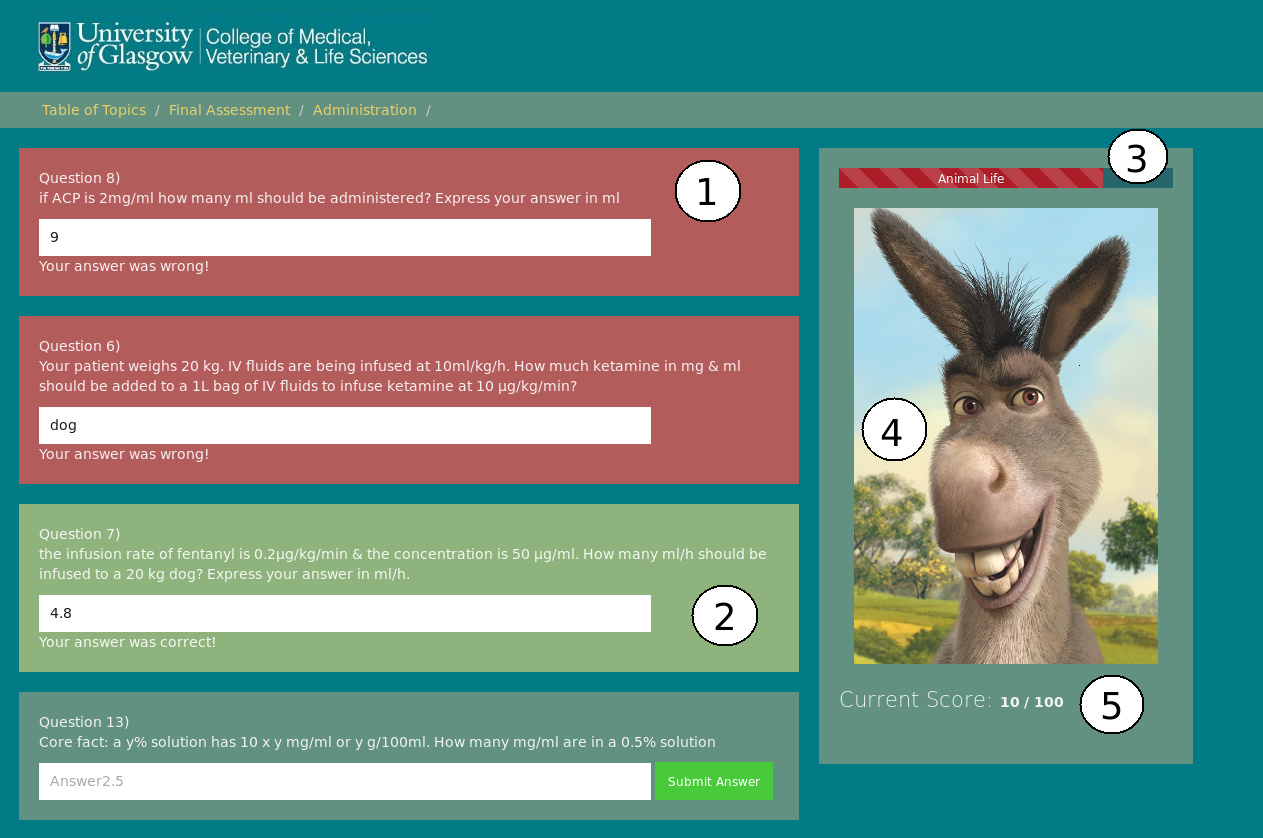
\includegraphics[width=\linewidth]{images/annotated_assessment.png}
\end{figure}

Figure 4.6 shows the assessment section of the application which presumably will be accessed when the user feels suitably prepared for it.

Annotation 1 shows an example of a question being answered wrong. Feedback is instantaneous with the question background changed to a subtle red colour, this is an intentional design decision to keep users engaged and willing to learn without discouraging them. Textual feedback is also provided for futher clarification. 

Annotation 2 shows an answer that is correct. This time the colour has changed to a slightly lighter green colour. Both the correct and incorrect colours are intrusive and fit with the design so as to keep the overall look pleasing.

The following three annotations illustrate the gamification of our application. By including the following elements we hope to engage users more effectively and provide an insentive to learn. Firstly they will attain a higher score and secondly they will keep the animal alive.

Annotation 3 is a progress bar which portrays the remaining health of the animal. For every wrong answer the bar will decrease indicating you hurt the animal (as a vet would do if they got these calculations wrong in the real world). Insentive to keep the animal alive will hopefully encourage the suer to get as many right answers as possible.

Annotation 4 is an image of the animal the students attempting to keep alive. For every decrement of 30 points the image changes to a steadily unhealthier looking donkey eventually resulting in a ``dead'' donkey. As with annotation 3 it is included to spur users to anser questions correctly.

Annotation 5 shows the users current score. This increases by ten points for every correct answer submitted and does not increase with wrong answers. 

\section{Conclusion}

The main focus of the design for the entirety of the application was to provide an interface that would be easy to use and reduce user frustration. Throughout development the idea of keeping users engaged with their learning and the content has been at the forefront and with the inclusion of a ``game'' of sorts on the final assessment the team believes they have succeeded in achieving this.

\chapter{Implementation}
\label{implementation}
\section{Developing a Web Based Application }
One of the requirements for our project was that our final product should be available to 
use to any user with an Internet Connection. More specifically, any student should be 
able to access the application and practice on their drug calculations in their free time 
wherever they are with any device that can access the Web. This can be a laptop 
computer, a mobile phone or a tablet computer. \\ 
It was, therefore, clear to us that creating an application that needs to be installed on a 
machine in order to be usable was not an option. After a discussion with the team we 
decided that the most suitable solution would be to implement a application that would be 
accessible via a Web Browser. A web application would make it possible for any user to 
access our application from any device simply by navigating to our Web Applications 
URL address. \\ 

\subsection {Using a Web Application Framework}
After doing some research looking for the best possible option for developing web 
applications we decided that we would make use of a web development framework 
rather than writing the code for the whole application from scratch.
\subsubsection{ Developing from Scratch}
Developing an application from scratch has the potential to take up much needed time 
from the Development Phase. For each different page of an application there needs to be 
a unique file (for example an html document) that will be sent to the client's web browser 
when the page is called. An application usually has the same layout on every page with 
basic components, like the applications logo or the applications default buttons, being 
displayed on each page. It is therefore clear that having a separate file to correspond to 
each different page of an application can lead to a lot of coding overhead and 'boiler 
plate' code. In the case of a change request, a developer will need to modify the code in 
each different page separately which would take much of our development time. Time was a major concern for us as we only had a limited amount of time to get the application designed, developed, evaluated and delivered to our client.
\subsubsection{Developing with a web application framework}
``A Web Application Framework is a set of prefabricated software building blocks that 
programmers can use, extend, or customise for specific computing solutions'' (Leif 
Azzoperdi, DIM3 Lecture 3). A framework would allow us to start implementing our 
application with a concrete base to support us by providing default functionality whilst 
allowing us to extend or override functionality to suit our specific requirements. ``One 
significant advantage to using a framework is that you're required to write only a 
minimal amount of code to get up and running from scratch''(Professional Python 
Frameworks: Web 2.0 Programming with Django and Turbogears page 48). This was 
one of the most important reasons for which we opted in using a Web Application 
Framework for our project. In addition, web appliccation freamworks support software reuse and component based programming which can help us separate concerns in our web application by breaking it down into different components. Afterwards, there was one more decision that needed to be 
undertaken. There are a number of frameworks available on the web so we had to decide 
on one of them before starting our implementation. 
\subsection {Which framework to use?}
We came down to three popular web application frameworks that would help us develop 
our software but we had to decide on one of them. Our supervisor suggested that three 
of us take one of the three frameworks each and try to build a simple application in one 
week. This would not only show us what can be built with that particular framework but 
it would also show us how long it take for a developer to learn how to use the 
framework, and how much can be built in a week by using that framework. The three 
options were 
\begin{itemize}
\item Web2Py 
\item Django 
\item Ruby on Rails 
\end{itemize}
After our frameworks evaluation we came to the following conclusions about them: 
Ruby on Rails offers useful code generators which can produce functions out of one line 
of code written by the developer and has a build in testing framework which can be 
particularly useful for our testing. However, the mystery behind the code generators can 
cause confusion to developers and thus increase development time. \\
Web2Py uses a Python-based template language and supports development from a Web 
Browser. We have been using python for our introduction to programming course in Level 
1 of our university studies so it would python is a language we have all used and are 
comfortable with. Moreover, a developer needs not have their own computer with them 
to work on the development of the application. Web2Py gives the ability to a developer 
to work on the code of the application via a web interface which can be particularly 
useful in case one of the team members is traveling and is not able to use their own 
computer to work on application. \\
Django is an MVT (Model, View, Template) based framework that runs with Python on 
its back end. This gives us the advantage of having separation of concerns in our 
application since different components in the framework act independently from each 
other so a developer can work on one part of the application while another can work on 
a different component without having to wait for a different component to be completed. 
Django is an extremely customisable framework since it comes packed with a lot of 
functionality which can be used out of the box or can be further modified to reflect our 
goals and objectives. On the other hand it might take time to learn since it has its own 
way of doing things and a developer needs to adapt to it.

\subsection {Why Django}
We decided to use Django since it gives us great flexibility as to what our end product 
can be like, it is documented extremely well online and even though learning it can take 
some time, we consider it to be a well worth investment since we will have to use 
Django in one of our courses in second semester as well. 
\section{Development in Django}
As its being described on djangoproject.org, Django is ``The Web framework for 
perfectionists with deadlines''. It is a rapid web development framework that can save 
you the trouble of writing repetitive boilerplate code. A developer using Django can 
achieve greatness with minimal coding. Django comes with an object relational mapper 
which means that we can define our database schema in Python code by defining 
classes and Django will then produce an sql code that can be injected in our database 
with minimal effort from the developer in order to create any tables required for the 
project. It has a dynamic build in administration interface which can be customised 
according to our needs. This can be used, in our case, as a way for a Course 
Coordinator or a Tutor to create new topics, add slides and questions to each topic, 
create questions for the final assessment page and create new users or groups of users 
with special permissions. This will be discussed further in this report.
\subsection{The MVT Model}
The MVT model used by django is a development mode very similar to the MVC model which is widely used by a number of web application 
frameworks such as Backbone.js SproutCore and the Cocoa framework used in Mac OS X and iOS applications. Django, since it likes to do things its own way, uses a ``modified'' version of the MVC model. Its model is called MVT (Model, View, Template). The model in the MVC 
plays the same role as the model in MVT which is sensible. However, the ``View'' in the 
MVT maps to the ``Controller'' of the MVC and the ``Template'' of the MVT maps to the 
MVC's ``View''. Of course this is slightly complicated so it might cause some confusion to 
a developer coming from an MVC background. 
The MVT in general defines the way everything works in Django. Everything in Django 
can be broken down to 3 components; The Models, the Templates and the Views.
\subsection{Models}
``A model is the single, definitive source of data about your data. It contains the essential 
fields and behaviours of the data you are storing''(Django website). In other words, any a 
table in the database can be created by defining a model in the Models.py file. A 
database field for that table can be defined as an attribute of the corresponding model. 
The command ``manage.py syncdb'' will then read the Models.py file create an SQL code 
and then run it agains the applications database to create any tables defined by the 
developer. 
For example if the code in picture below is run it will create a Database table of topics 
where each topic has a title and a publication date. \\
class Topic(models.Model): \\
title = models.CharField(max\_length=100) \\
pub\_date = models.DateTimeField('Date Published')\\
\subsection{Views}
A view takes care of what is sent to a browser when a specific URL is requested. It is 
responsible for making any requested action as this is defined in the tags of the html 
page associated with each view. Such actions might be read or write to the database 
commands or any other actions that are required by a page.
\subsection{Templates}
A template is usually an html file. It is the base of what will be send on to a web browser 
client. It described how the data should be presented to the user and can contain a 
number of Django tags and variables. A tag is surrounded by ``'' and tells 
Django that a special action needs to be taken at that point of the page. This special 
action can be an ``if'' statement, a ``for'' loop etc. A variable is simply telling Django to load 
a specific value from the Database and display it at this point of the page. Templates are 
used by Django as the model for a page to be sent to a web client.
\subsection{Controller}
Each Django application has a ``urls.py'' file which holds definitions that will be matched 
against requests by web clients. An example url definition in ``urls.py'' could be \\
\verb|``url(r ^'contents', 'views.contents')''|. \\In this scenario if our server is hosted on 127.0.0.1 
port 8000 and a client requests ``127.0.0.1:8000/contents'' Django will match the 
request with the definition in ``urls.py'' and call the appropriate view which is the second 
argument of the url() function. In this case it will be the ``contents'' view.
\section{3-Tier Architecture}
For our implementation we used a 3-Tier Architecture.
\begin{figure}[!htb]
\caption{3-Tier Architecture Diagram}
 \centering
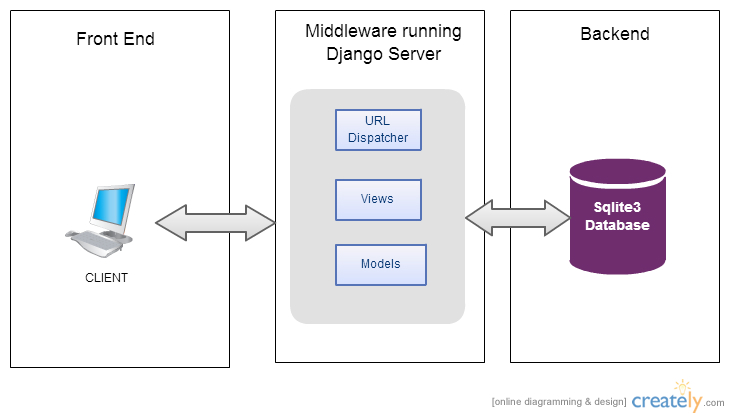
\includegraphics[width=0.9\textwidth]{images/ntier.jpg}
\end{figure}
\subsection{Front End}
The application can be accessed by any user with a web browser such as Internet 
Explorer, Google Chrome, Mozzila Firefox, Safari and so on. \\
\subsection{Middleware}
This is our Django server. Responsible for matching requests from Clients using the 
URL dispatcher which in return calls the appropriate View which then fetches any 
required context from the Models.py and our Backend Services. 
\subsection{Back End}
This is our Sqlite3 Database. Other database options included MySQL, Oracle or 
PostgreSQL. However we opted in for Sqlite3 since it offers all the functionality we 
need and Django provides more support for it as it is its default option. \\
\section{Back End - Data Models}
Our database consists of 4 basic data models. Namely, Topic, Question, FinalTestQuestion and Slide. According to our requirements, a Topic can have 0 or more questions and slides. Thus, the Question and Slide objects both have a foreign key that points to the Topic they belong to. More information on the definitions of our Data Models can be seen in the tables below: 
\subsection{Data Model:Topic}
\begin{tabular}{|c|c|c|}
\hline \textbf{Field Name} & \textbf{Type} & \textbf{Notes}\\
\hline title & CharField & 1000 characters max \\ 
\hline pub\_date & DateTime &  \\ \hline
\end{tabular}
\subsection{Data Model:Question}
\begin{tabular}{|c|c|c|}
\hline \textbf{Field Name} & \textbf{Type} & \textbf{Notes}\\
\hline qTopic & ForeignKey & Points to a Topic object \\ 
\hline text & CharField & 1500 characters max \\
\hline answer & CharField & 100 characters max \\ \hline
\end{tabular}

\subsection{Data Model:FinalTestQuestion}
\begin{tabular}{|c|c|c|}
\hline \textbf{Field Name} & \textbf{Type} & \textbf{Notes}\\
\hline text & CharField & 2000 Characters max length \\ 
\hline answer & CharField & 100 characters max \\ \hline
\end{tabular}

\subsection{Data Model:Slide}
\begin{tabular}{|c|c|c|}
\hline \textbf{Field Name} & \textbf{Type} & \textbf{Notes}\\
\hline sTopic & ForeignKey & Points to a Topic object \\ 
\hline image & ImageField &  \\ \hline
\end{tabular}

\section{Managing the Front End}
The way Django is generally managing the Front End of an application is quite 
straight forward. It simply takes a predefined template (html file), adds any required 
content from the models (database objects) and sends the file over to a web browser. 
However creating simple html files and feeding them the data from our models is not 
enough to produce a high quality web application. Producing a rich interactive user interface was extremely important in our case since the application would be used by students to assist their studying. Students can easily get tired of studying and abandon their task so we had to make the interface as attractive as possible, in the little time we had, so that a user can stay motivated and enjoy using it the application.The fact that we were not 
experienced in web application was not helping us find a solution without investing 
some time on researching. In our quest to find a way to manage the front end design 
we looked at a number of solutions. Some of them were the ``Backbone.js'', ``Tastypie'' 
and ``Pyjamas''. At a first glance each of these frameworks seemed promising. 
However, trying to use them to produce high quality front end design became more of 
a time wasting challenge rather that a time worthy investment.
\subsection{Possible frameworks for Front End management}
\subsubsection{Backbone}
As its website states, ``Backbone.js gives structure to web applications by providing 
models with key-value binding and custom events, collections with a rich API of 
enumerable functions, views with declarative event handling, and connects it all to 
your existing API over a RESTful JSON interface''. Fair enough, now how can we 
proceed and use this Framework with our Django application? A number of github 
repositories were available online, all with example applications using Backbone. 
However, since all of them were out of date and description for Backbone and 
Django integration was vague at best, we soon abandoned the idea of using 
Backbone. 
\subsubsection{Pyjamas}
Pyjamas is a framework which takes code written in Python and translates that 
into javascript and jquery code without the need of having a developer experienced 
in using javascript and jquery. We managed to get Pyjamas set up successfullly, 
but the result was not exactly what we expected. The design looked poor and we 
had to invest even more time in advancing our skills on coding a GUI with python
\subsubsection{Compination of traditional Django friendly frameworks}
Luckily for us, one of our team members who is really confident on his web design skills
convinced us that surely using traditional web design methods, such as writing the code for the templates directly in javascript and using a simple collection of tools such as the Twitter Bootstrap might be worth looking into. He suggested that he can try work out a first draft of the Topics page so that we can see what he can produce with these tools and judge for ourselves. Creating the page actually took him less than one hour and that was a wakeup call for us since the sample page he created was both looking aesthetically nice and the technologies used were working with the Django seamlessly with minimal effort.  
We started by creating a base.html template. Django gives a developer the option to create templates that inherit from other templates. So any code that needs to be repeated in every page needs not be defined more than once. Our  base page with no additional content can be seen on figure 1.2 .
\begin{figure}[h!]
   \caption{Base.html Template}
   \centering
     
\includegraphics[width=0.6\textwidth]{images/base.jpg}
\end{figure}
This includes the basic layout that should be displayed on ALL templates of our application. So to make the connection between our base template and all other template we had to define an empty Django tag  called “content block” in our base.html template (see figure 1.3). 
\begin{figure}[h!]
   \caption{The Base.html template with no additional content}
   \centering
     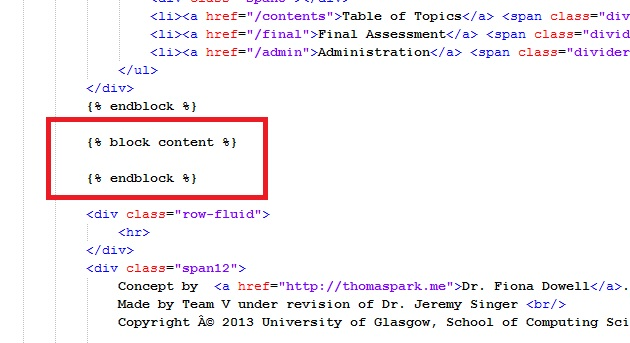
\includegraphics[width=0.6\textwidth]{images/baseblock.jpg}
\end{figure}
Then on every page that needs to inherit from base.html we can define the content block so that it includes any additional data that each specific template may require. An example of how a block is defined in a base template is shown in figure “baseblock.jpg” and then the way the base template is inherited and the “content block” is used can be seen on figure ``extendsbase''.
\begin{figure}[h!]
   \caption{Contents template inherits from base.html.}
   \centering
     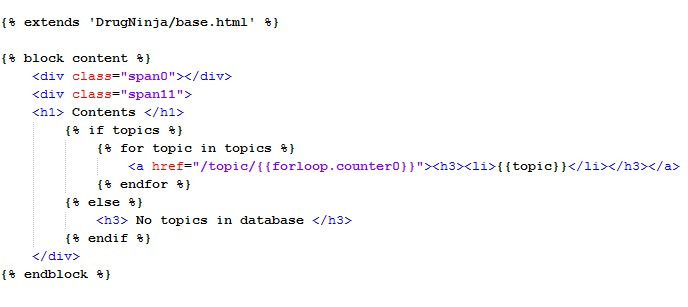
\includegraphics[width=0.7\textwidth]{images/extendsbase.jpg}
\end{figure}

\section{Middleware: Linking the back with the front}
Django makes the connection between the backend data models and the front end templates by interpreting a request from a web client, finding the required template for that request and rendering the context on the page by replacing all Django tags (text surrounded by '{\%' and  '\%}') with data returned by the responsible view for that request.  For  instance, figure **contentsView** shows how the contents View is defined. The tag “topics” is declared as a list of Topic objects and then by adding the key “topics” into the contents view context we are telling the view to return the list “topics” every time the tag “topics” is found on the template “contents.html”. Then in template “contents.html” we make use of a for loop to iterate through the topics list, and print out the topic name with a link to its unique url. After the template has been rendered it is sent on to the web browser where it is presented to the urer who requested the page.
\section{Message Passing}

\subsection{Database Request Format}
Database Requests are handled by Django. A template may require information about a specific data model. The view that makes use of that specific model makes SQL request to the database which in turn returns any matching results from our SQLite database.
\begin{figure}[h!]
   \caption{Database Request figure}
   \centering
     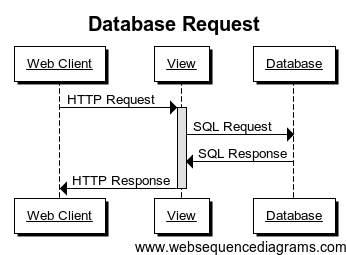
\includegraphics[width=0.5\textwidth]{images/databaseMessagePassing.png}
\end{figure}

\subsection{Answer Validation Request}
The validation of answers is done by an Ajax request to  the “validateAnswer” view or to the “validateFinalAnswer” view when the answer to be validated belongs to a final assessment type question. The validation is done by passing the question id and the provided answer as URL parameters. The view  then makes a request to the database requesting the answer of the required question. If the answer provided by the user is the same as the one stored in the database the view will respond to the web client with an appropriate Http Response as on figure 1.6.
\begin{figure}[h!]
   \caption{Answer Validation Request figure.}
   \centering
     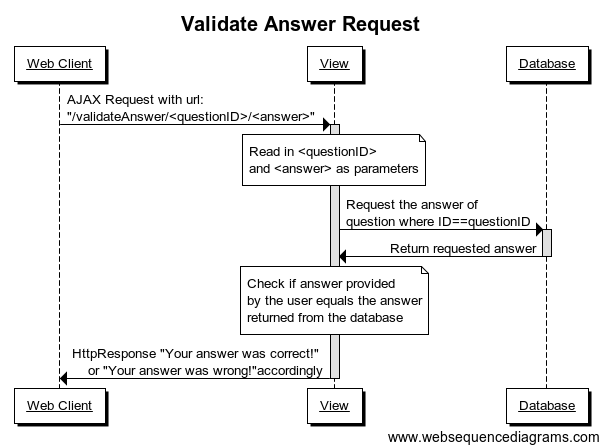
\includegraphics[width=0.6\textwidth]{images/validateAnswerRequest.png}
\end{figure} 

\subsection{Topic Related Data Request}
Topic requests make use of the “Topic” view. The view uses the “topic.html” template and renders it so that it gains access to a list of Topic objects. When, for example, a user needs to navigate to the appropriate page for the first topic in the Topic objects list, they should navigate to “/topic/0” where 0 is the position of the first Topic objects in the topics list. When the slides of a specific Topic need to be displayed, a “for” loop is used to iterate through the list of slides and return only those that point to the Topic that was originally requested by the URL.

\begin{figure}[h!]
   \caption{Topic Related Request}
   \centering
     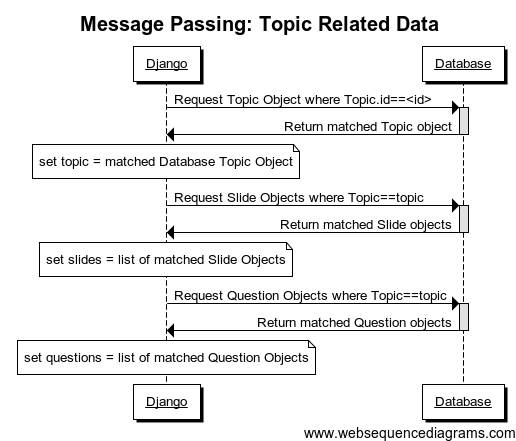
\includegraphics[width=0.7\textwidth]{images/topicRelatedRequest.png}
\end{figure} 

\section{End Product}
\subsection{Desired Functionality}
The Desired Functionality section aims to describe how the desired functionality mentioned in Requirements and Design sections was realised through the implementation will now be demonstrated in more detail.

\subsubsection{Welcome Page}
The welcome page is implemented through the “index” view.  It is maybe the simplest template in our project. It is a simple template that inherits from base.html and includes a static text with a brief description of our web application and a button that points to the first topic page.
\begin{figure}[h!]
   \caption{Final Welcome Page}
   \centering
     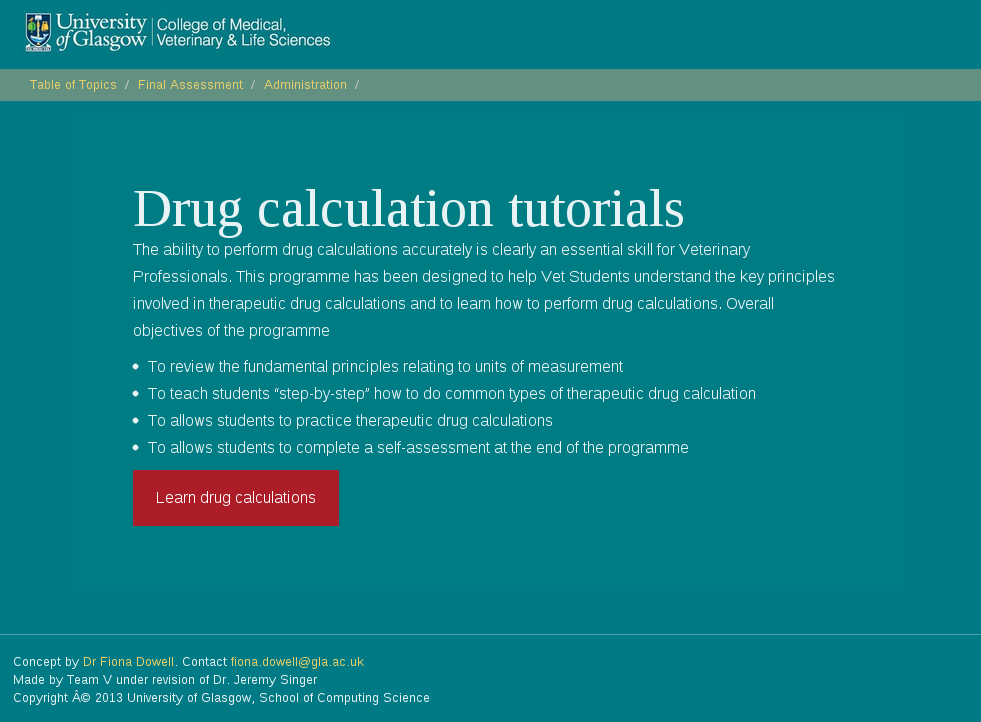
\includegraphics[width=0.7\textwidth]{images/welcomePage.png}
\end{figure} 

\subsubsection{Topic Page}
The topic page consists of two equal width side bars. The left sidebar is a carousel which displays all the slides related to each topic and the right sidebar  consists of a “for” loop that displays all the questions related to each topic along with a text box for a user to enter their answer and a submit button. Once a submit button is pressed, an ajax call makes a request to the server which responds with a “correct answer” or “false answer” accordingly.  The response from the database updated the string on the submit button so the text on the button changes from “Submit” to “Correct answer” or “False answer”.
\begin{figure}[h!]
   \caption{Topic Page}
   \centering
     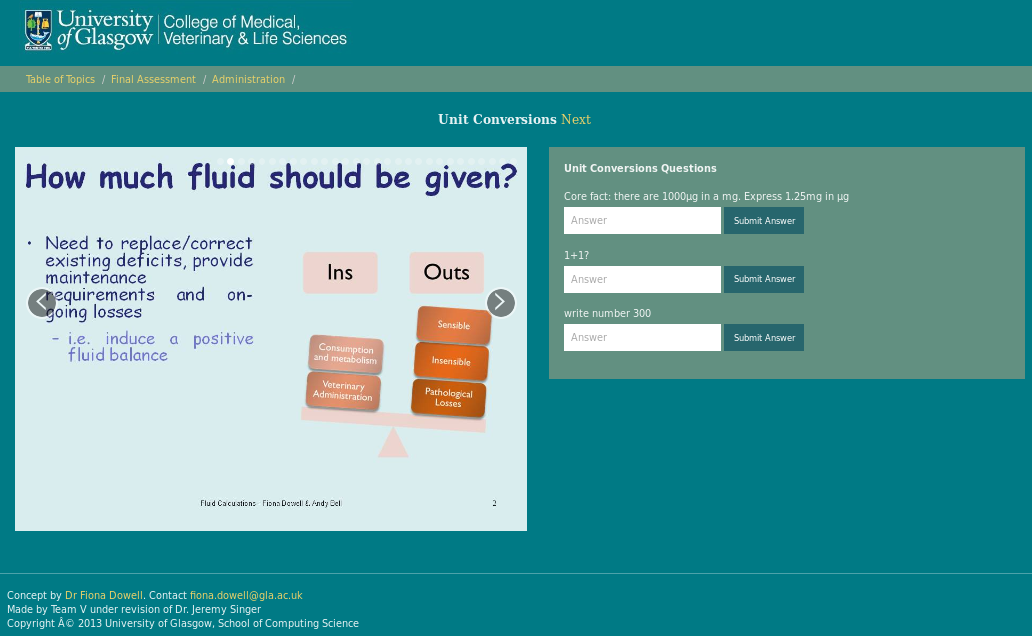
\includegraphics[width=0.7\textwidth]{images/topicPage.png}
\end{figure} 

\subsubsection{Contents Page}
The contents page is implemented so that a user can navigate directly to a specific topic page without having to go through all other topics via the “Next” button on each topic page. A “for” loop is used on “contents.html” template which is used so that the “contents” view will replace the contents of the “for” loop with a list of all Topic Names currently stored in the database with links that point to that specific Topic’s page.
\begin{figure}[!htb]
\caption{Contents Page}
 \centering
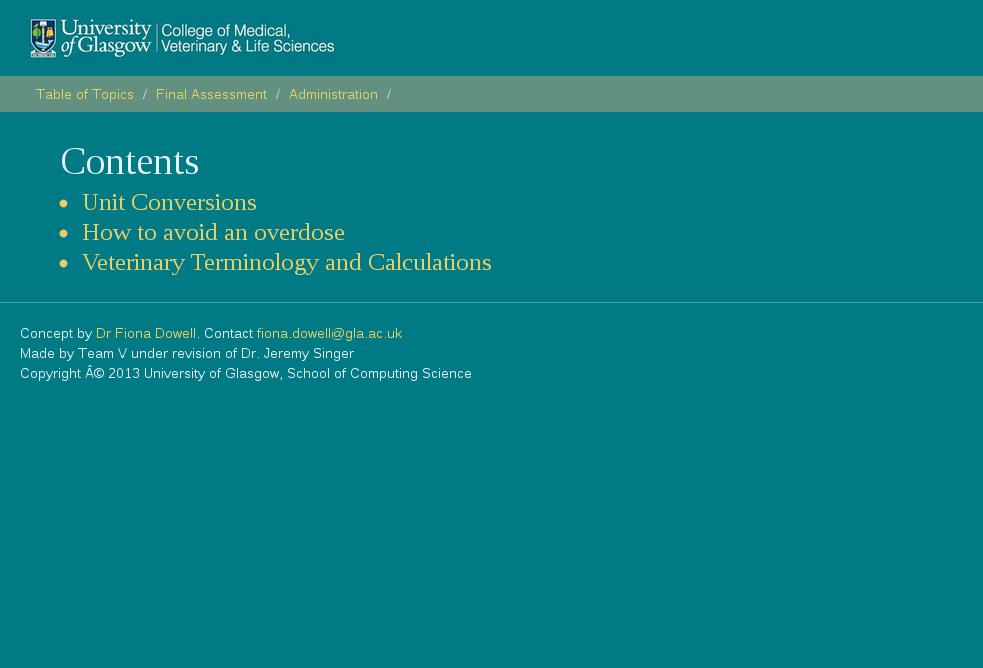
\includegraphics[width=0.9\textwidth]{images/contentsPage.png}
\end{figure}

\subsubsection{Final Assessment Page}
The final page is one of the core components of our application. The requirements were clear. A user should be faced with 10 random questions from the “FinalAssessmentQuestion” database model and he or she should only be allowed to have one attempt to answer the question. This is to make sure that a user pays the required amount of thinking before clicking the “Submit Answer” button. Our client initially provided us with a number of sample lecture slides so that we could get an idea of her lectures’ contents. We noticed that a picture she uses often to make her lecture slides more interesting to students is a picture of “donkey” from the Shrek movies. So we thought that since the users are probably already familiar with the Shrek donkey so we added it on a side bar in an attempt to make the Final Assessment Page more interesting and appealing to the users. We also added a “health bar” and a “Score” label. The score label has a maximum value of 100\% and it defaults to 0\% while the “health bar” has a maximum value of 100\% but defaults to the maximum. Each time a user enters a value to a questions text box and clicks the “Submit Answer” button an Ajax request is sent to the Django server which responds with “Correct Answer” or “False Answer”. If the answer was correct, the Score label will be update with the current score + 10 and the health bar will not be modified. However, if the answer was wrong the value of the health bar will go down by 10\% and the score will remain the same.  In addition, if the value of the health bar falls below 50\%, the image of the donkey will change from the default “happy donkey” to a “sad donkey” and then if it falls below 1\% an alert will be displayed to the user with a “You have killed your animal” notification and the picture of the donkey will be changed to a dead donkey.  A colour coded response is also displayed to the user as the question box turns red if the users answer was wrong, or green if the users question was correct. 
\begin{figure}[!htb]
\caption{Final Assessment Page}
 \centering
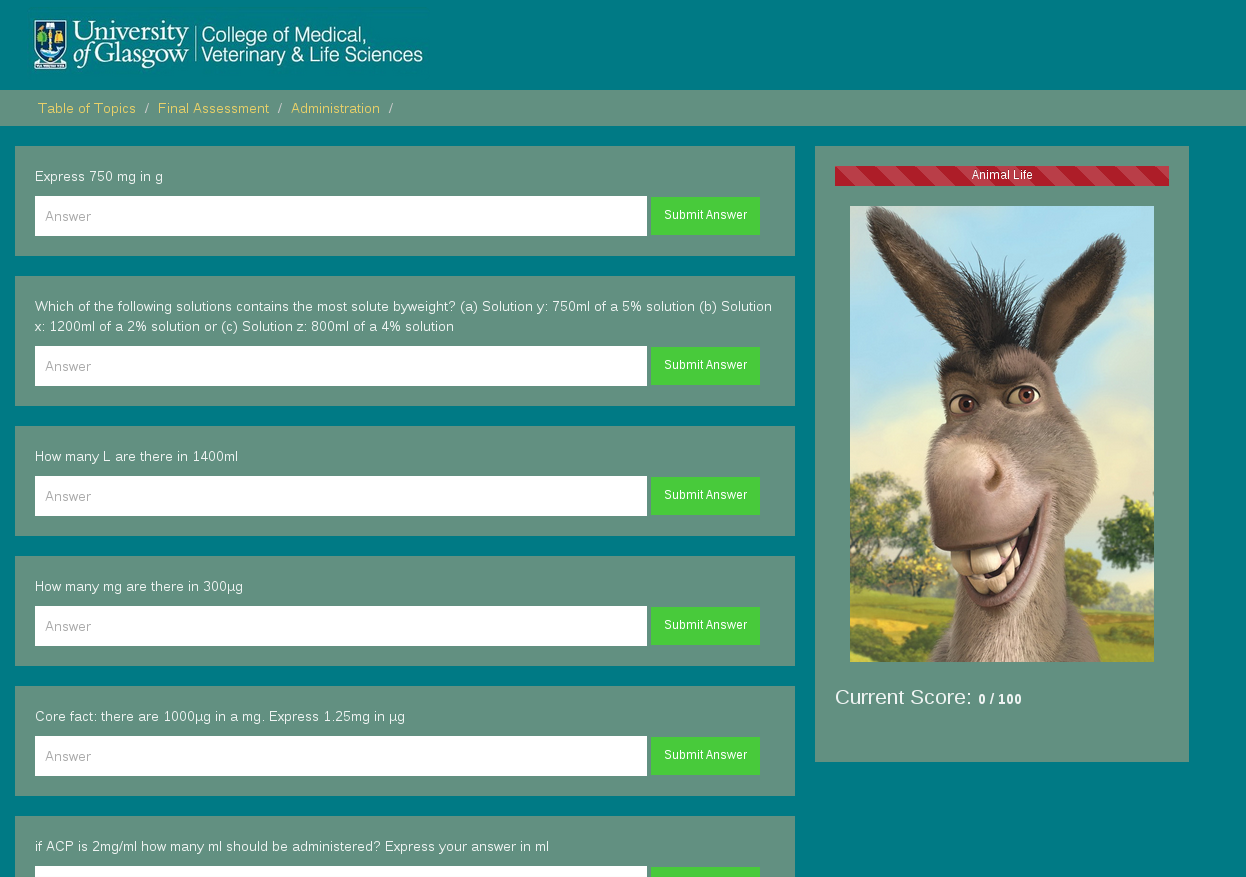
\includegraphics[width=0.9\textwidth]{images/finalAssessmentPage.png}
\end{figure}
\subsubsection{Administration Page}
The administrator page is dynamically created by Django. We only needed to define which models needed to be modifiable from the admin page and the  way we want them to be displayed.  Two groups of modifiable data models were defined. “Topics” and “FinalAssessmentQuestions”. The reason behind this was that questions and slides have a foreign key that points to a Topic so by selecting a Topic in the administration page a user can see and modify all slides and questions that are related to that Topic. By navigating to the “FinalAssessmentQuestions” a user can add, delete or modify a Final Assessment Question. By default, Django also provides a user management interface by which  a user with administrative rights can manage users by adding, removing or modifying permissions for other users.The administration home page can be seen in Figure 1.4 and the Modify Topic interface in Figure 1.5
\begin{figure}[!htb]
\caption{Administration Home Page}
 \centering
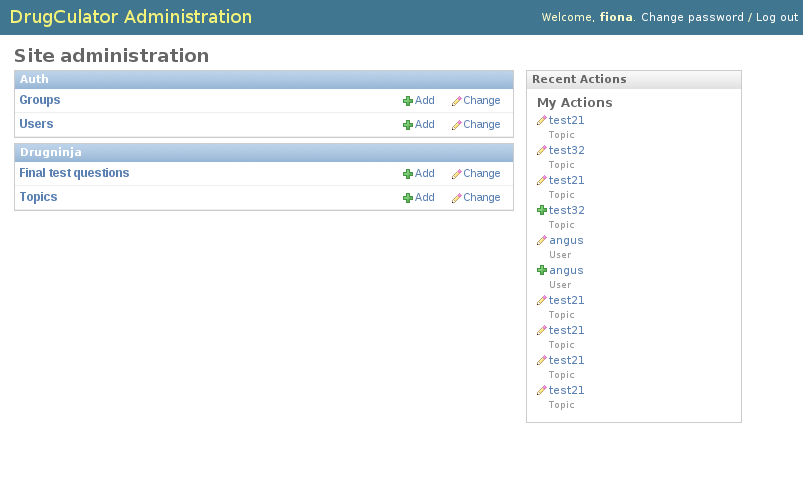
\includegraphics[width=0.9\textwidth]{images/adminPage.png}
\end{figure}

\begin{figure}[!htb]
\caption{Modify Topic Interface}
 \centering
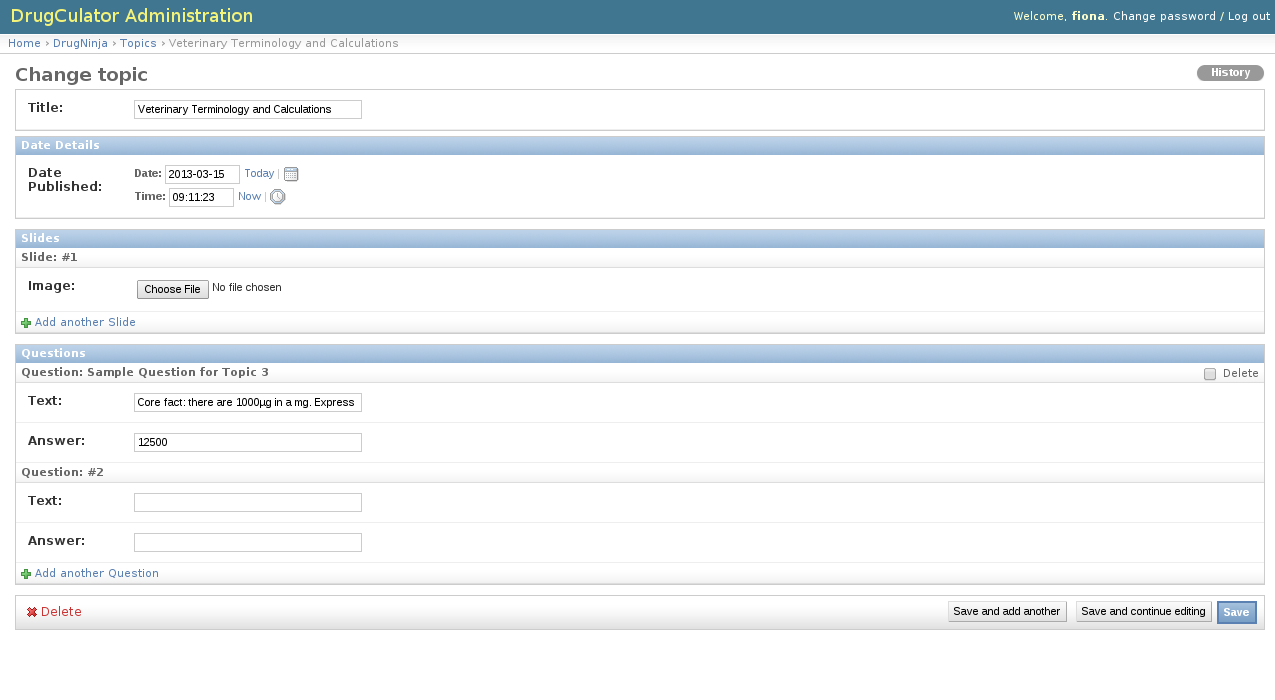
\includegraphics[width=0.9\textwidth]{images/adminTopic.png}
\end{figure}

\subsection{Interaction Diagrams}
\subsubsection{Topic Page}
Interaction diagram for communications and message passing between Topic Page and the server
\begin{figure}[!htb]
\caption{Topic Page Interactions}
 \centering
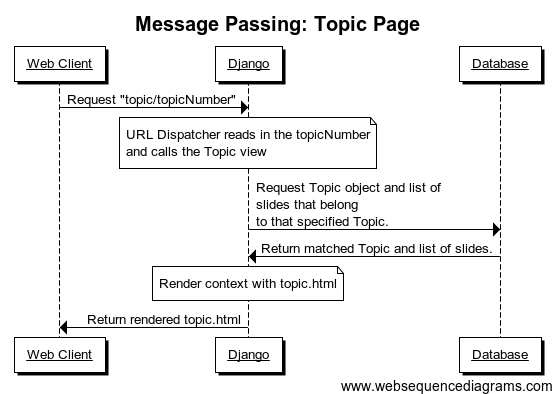
\includegraphics[width=0.9\textwidth]{images/topicPageMessagePassing.png}
\end{figure}

\subsubsection{Contents Page}
Interaction diagram for communications and message passing between the Contents Page and the server
\begin{figure}[!htb]
\caption{Contents Interaction Diagram}
 \centering
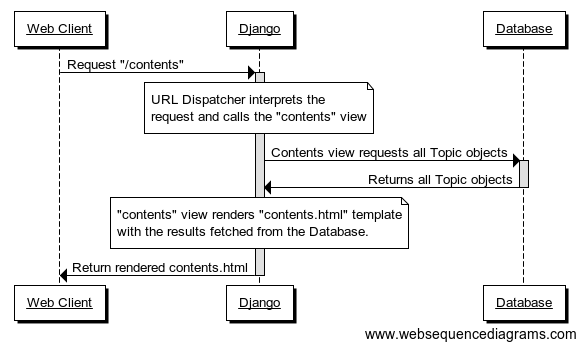
\includegraphics[width=0.9\textwidth]{images/contentsInteractionDiagram.png}
\end{figure}

\subsubsection{Final Assessment Page}
Interaction diagram for communications and message passing between the Final Assessment Page and the server
\begin{figure}[!htb]
\caption{Final Assessment Interaction Diagram}
 \centering
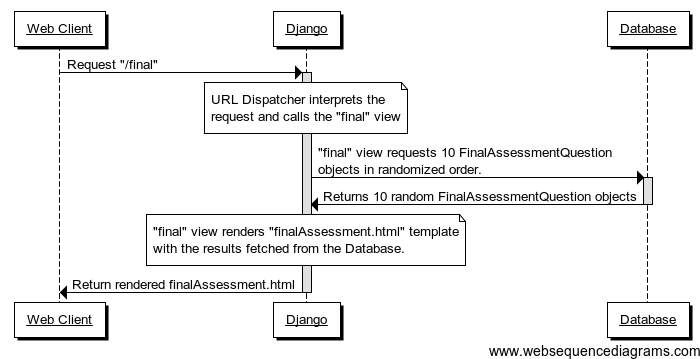
\includegraphics[width=0.9\textwidth]{images/finalAssessmentInteractionDiagram.png}
\end{figure}
\section{Challenges and Solutions}
\subsection{Referencing topics by topic.id}
When we first started working with topics we were using the topic ids provided by Django to reference and call topics from a template's perspective. However we soon realised that Django was using the IDs provided by SQL and not some IDs that were generated by Django. The result of this error on our behalf was that when a Topic was removed from the database, the ID numbers for topics were not automatically regenerated so clicking the next button (this calls topic with topic ID equal to the current topic's ID+1) on a Topic page would call a Topic ID that might not exist in the database. Consequently, that would cause the application to run on an Index error In order to bypass this issue, we looked at alternative ways of indexing the list of Topics and returning available Topic numbers.  Instead of using Topic IDs we started using Topic List positions. More specifically, we are now creating a list of Topics in Topic view by requesting ALL the Topics currently held in the Database and then iterate over that one. For example, when “/topic/0” is called, instead of requesting Topic with TopicID==0 from the database, we are requesting the Topic in position [0] of our runtime created Topic list. This way, the numbers used to request topics are always up to date with exactly what's currently held in the Database.  We have also added checks to see whether the current topic is the first or last topic in the Topics list. In which case the “Next” or “Previous” buttons are hidden accordingly.

\subsection{URL Dispatcher for Validating Questions}
As mentioned in previous sections, the way we validate answers is by passing them as parameters with an Ajax Request.  The URL dispatcher then matches the url the web client requests and matches that with the ``validate'' url definition in urls.py. The url definition for ``validate\_answer'' is: \verb|``url(r'^validate_answer/(?P<question>\w+)/(?P<answer>\w+)|', 'views.validate')''. By definition \verb|(?P<answer>\w+)| accepts any string as answer. However when a user provides an answer such as “2.5”, the URL dispatcher accepts “2” and disgards anything after the decimal point. This was causing answer validations to fail even when the answer provided by the user was correct. The Django documentation on URLs was not particularly helpful so through a process of trial and error we arrived at a valid solution that can match both strings (this can be a non decimal number as well) and decimal numbers. In addition to our \verb|“url(r'^validate_answer/|\\\verb|(?P<question>\w+)/(?P<answer>\w+)'|, 'views.validate')” regular expression we added \verb|“url(r'^validate_answer/|\\\verb|(?P<question>\\w+)/(?P<answer>\\d+\.\\|d+)', 'DrugNinja.views.validate')” right before the first expression. In essense, when a validate answer request arrives, the URL dispatcher will try and match it to the new reqular expression which only matches answers with a decimal point. If the answer does not match, Django will try to match it to the second URL definition which accepts strings or non decimal integers and respond accordingly.

\subsection{Static Files}
Django has some strict safety rules when it comes to static files. When we started our implementation, having only basic web design knowledge, we though that defining a static files directory would be enough for Django to be able to write and read files. This seemed to be the case since when we were uploading images to the system through the administration interface, the system seemed to be reading the files just fine and saving them in the correct directory. However, when a web browser made a request for a static file Django was returning 404 errors referring to a local file that we were sure that exists. This made absolutely no sense to us so resolving this error was particularly time consuming. After a lot of research in Django's Documentation we found out that Django does not allow a web browser to access the static files directory directly. A new directory should be defined as public in Django settings file. This way, a browser would make calls against the public directory and even though that directory is empty, Django will copy files to it and make them accessible to the web browser without making the original files valnurable to malicious activity by a web client user.
\section{Known Issues}
There are currently two known issues in our application which are planned to be resolved after this release.\\
\begin{itemize}
\item Font can be different from web browser to web browser.
\item The slides carousel behaviour is slightly different when accessed through Google Chrome. This is not a serious issue and does not affect the user experience in any major way.
\end{itemize}

\chapter{Evaluation and Testing}
\label{evaluation}

This section discusses the methods used for testing and evaluating our application. Testing is important in order to ensure that all requirements are met and to identify and rectify any errors. Using various methods of evaluating allows us to test the usability and functionality of our final application.

\section{Testing}

\subsection{Test Plan and Strategy}

Firstly, we created a test log in which we added the feature tested, the date it was tested and the result of the test. Each time we tested a new feature it was added to the test log in order to keep track of what had been tested and whether or not it had been successful.

Initially, for testing our application, we tested each new feature as they were implemented. After running the application to see if the new feature worked as expected, we then tested it with the previous feature already implemented to ensure that they didn't conflict or cause the application to crash.

If an error was detected or the feature caused the application to crash, this was documented in the test log and was raised as an issue on the team's GitHub. It was then assigned to a developer so that the issue could be diagnosed and fixed. Doing this allowed us to keep track of any and all issues and errors that had occurred throughout the implementation process.

However, we found that this was very time consuming, as opposed to having a pre-defined set of test scripts. We then created a set of test scripts for each page within the application. After implementing several features, we would run the test-script in order to see if they worked as expected and produced the correct output.\\
This will give us a generic view of our application's status. This would dynamically generate a pie chart to give a visual presentation of the number of 'Passed', 'Failed' and 'Blocked' tasks.

\begin{itemize}
\item Passed Result - a test task that runs successfully and produces the expected result.
\item Failed Result - a test task that does not produce the expected result.
\item Blocked Result - A test task that cannot be run, due to an issue thats waiting to be resolved. For example, if the answer validation function is not yet implemented, then a test that includes answer validation cannot be run.
\end{itemize}

\subsection{Issues}

Some of the main issues we encountered are listed below.

\begin{center}
Table 6.1 - Main issues occurred throughout development\\
\begin{tabular}{|c|c|}
\hline \textbf{Issue} & \textbf{Current Status}\\
\hline 
\hline ImageField throws 404 error when trying to access saved Image & Resolved\\
\hline No error for 0 slides in a topic & Resolved\\
\hline Application crashes when clicking next topic button & Resolved\\
\hline Application font appears different on different web-browsers & Unresolved\\
\hline System returns ``Wrong answer'' for correct answer. & Resolved\\
\hline Questions in final assessment are not displayed in random order & Resolved\\
\hline
\end{tabular}\\
\textit{{\small The table shows some issues which we encountered throughout the development of our application.}}
\end{center}


% Bugs 
% ImageField throws 404 error when trying to access saved Image
% No error for 0 slides in a topic
% Topic id not updating - had to use a topic list.

\subsection{Testing Results Sample}

An example test script can be seen in Figure 6.1 This includes a set of tasks with their expected behaviour and the results achieved in each test cycle. 

\begin{figure}[!htb]
\caption{Test Script Example}
 \centering
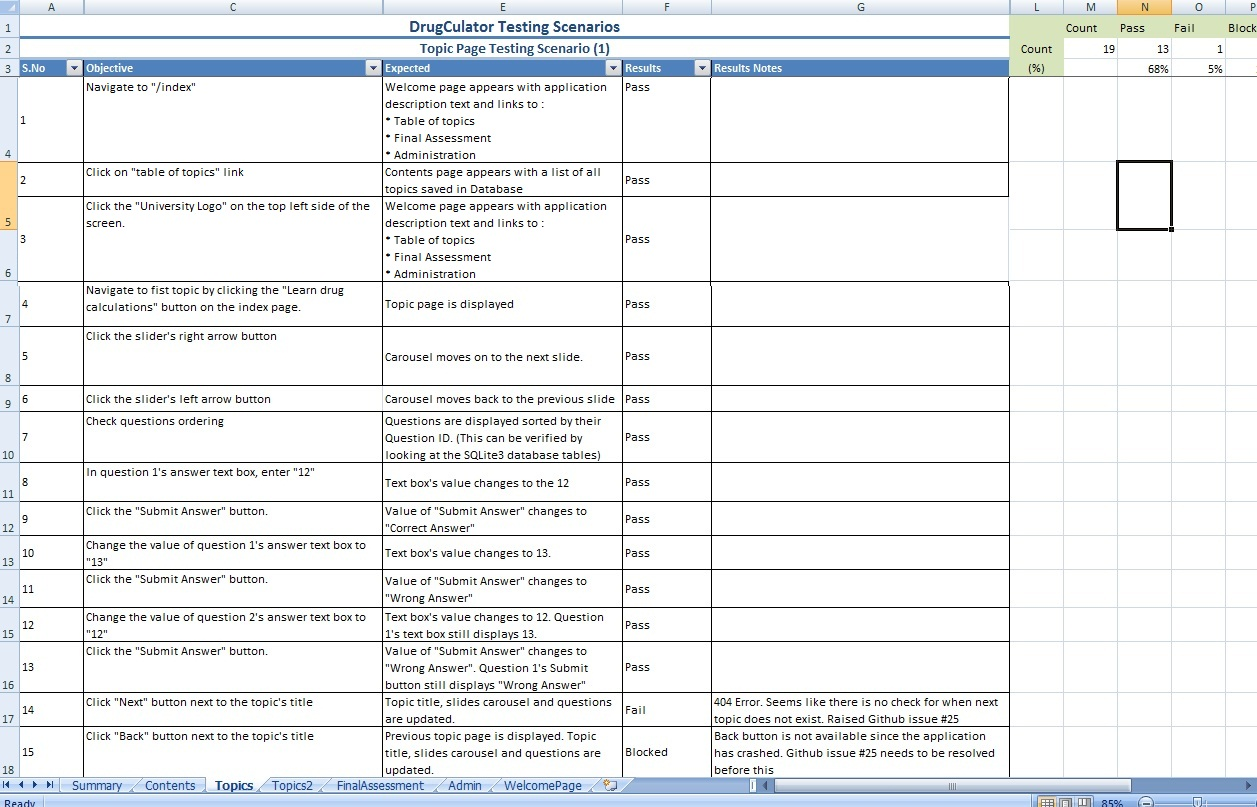
\includegraphics[width=0.7\textwidth]{images/TopicTest.jpg}
\end{figure}


Figure 6.2 below shows the test results summary for all the test scripts produced. 

\begin{figure}[!htb]
\caption{Test Results Summary Example}
 \centering
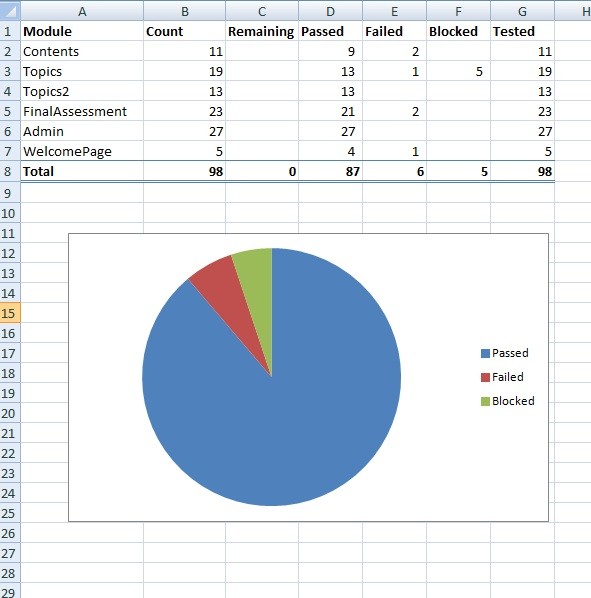
\includegraphics[width=0.5\textwidth]{images/TestResultsSummary.jpg}
\end{figure}

\section{User Evaluation}

In order to test the usability and functionality of our application, we identified the features of the application which would provide us with the most accurate results:

\begin{itemize}
\item Content management: admin users should be able to easily upload, edit and delete content.
\item Browse through topics successfully.
\item Answer all questions available.
\item Complete the final assessment and see their final score. 
\end{itemize}

We then created a test plan to evaluate the usability and aesthetic appeal of the application. To test both the administration features and the learning functionality for the students, we created a set of tasks based on the features above. We used the 'Think-Aloud' method during the evaluation and provided participants with a short questionnaire afterwards.

\subsection{Functional Requirement Fulfilment}

%At this point in time all of the client's requirements have been met. This application's implementation has been very iterative.
%Meeting with our client repeatedly over the course of development has meant that we have been steadily improving the application and refactoring our code. 
%
%Developing beyond the must have requirements we have developed a game-ified final assessment page and also refined our application design to increase usability and aesthetic appeal for the end user.

Before carrying out our evaluation with a group of participants, our team carried out an evaluation on ourselves in order to test the application for issues and to see how many of the requirements were satisfied. From this evaluation, we found that our application satisfies each of the client's 15 specified functional requirements. The admin user is able to upload new content, edit and delete content. The student user can view all topics available and see all related slides and questions for each topic. The student user can also complete the final assessment and see their final score, indicating how well they answered.

The application's implementation has been a very iterative process, and meeting with our client repeatedly over the course of the development has meant that we have been steadily improving the application and refactoring our code.

Developing beyond the `must have' requirements, we have developed a game-like final assessment page and also refined our application design to increase usability and aesthetic appeal for the end user.


\subsection{Users}

Firstly, we wanted to do an evaluation with our client: Dr Fiona Dowell. This would allow us to see how satisfied our client was with the application we had created and allow us to receive any feedback. Following that, we wanted to get a mixture of Computing Science/Software Engineering students and other students to evaluate our application. As the Computing Science/Software Engineering students had done coursework with Django recently, we thought that having participants who are unfamiliar with Django would provide us with more reliable results for our evaluation.

\subsection{Tasks}

We asked the participants to carry out a number of tasks in order to evaluate our application. We have tasks for both an admin user, to test the administration features and content management, and for a student user, to test the functionality and usability of the learning features.
\newpage

\textbf{Admin User Tasks}

\begin{center}
Table 6.2 - Admin User Tasks
\begin{tabular}{|c|c|}
\hline & \textbf{Task}\\
\hline 1 & Login as administrator.\\
\hline 2 & Add a new user.\\
\hline 3 & Set the users permissions to allow them to update content - topics, slides, questions.\\
\hline 4 & Add a new Topic.\\
\hline 5 & Add a new slide to that topic.\\
\hline 6 & Go to Topic 2 and remove slide 3.\\
\hline 7 & Add a new question to Topic 1.\\
\hline 8 & Edit question 2 within Topic 2.\\
\hline
\end{tabular}\\
\textit{{\small This table shows the tasks to be carried out by partipants in order to evaluate the admin user functionality.}}
\end{center}

\textbf{Student User Tasks}

\begin{center}
Table 6.3 - Student User Tasks\\
\begin{tabular}{|c|c|}
\hline & \textbf{Task}\\
\hline 1 &  Go to Topic 1 and browse through the slides.\\
\hline 2 & Answer 2 questions within Topic 1.\\
\hline 3 & Go to Topic 2.\\
\hline 4 & Go to the final Assessment and complete the test.\\
\hline
\end{tabular}\\
\textit{{\small This table shows the tasks to be carried out by participants in order to evaluate the student user functionality.}}
\end{center}

\textbf{User Consent}

In order to avoid any ethical issues, all participants were issued a consent form, which informed them what the testing would involve and what exactly it was for.  It also stated that the participant information would be kept private and that they are able to leave the testing at any time if they did not wish to continue. The consent forms had to be signed and returned before any testing was allowed to commence.

\textbf{Think-Aloud}

All evaluations were performed using the Think Aloud method which involves observing the participants performing the tasks and having them describe out loud what they are doing and why. This is a useful evaluation method as it allows us to see first-hand the process that the participants go through to complete the tasks and highlights any difficulties or errors they may encounter.

\textbf{Questionnaire}

After the evaluation, each participant was asked to complete a quick questionnaire about the application and the tasks they had completed, and provide any additional feedback. The first 4 questions are related to the usability of the content admin tasks, and questions 5 to 8 are about the usability of the student user tasks.

\begin{center}
Table 6.4 - Questionnaire\\
\begin{tabular}{|p{2cm}|p{12cm}|}
\hline & \textbf{Questions} \newline \newline Key: 1 - very easy; 5 - very difficult \\
\hline 1 & Overall, how easy was the admin system to use? \newline 1 ~~~~~~~~~~ 2 ~~~~~~~~~~ 3 ~~~~~~~~~~ 4  ~~~~~~~~~~ 5\\
\hline 2 & How difficult did you find it to add a new user to the system?  \newline 1 ~~~~~~~~~~ 2 ~~~~~~~~~~ 3 ~~~~~~~~~~ 4  ~~~~~~~~~~ 5\\
\hline 3 & Were you able to change a user's access permissions? If so, how difficult was this?  \newline 1 ~~~~~~~~~~ 2 ~~~~~~~~~~ 3 ~~~~~~~~~~ 4  ~~~~~~~~~~ 5\\
\hline 4 & How easy was it to add new content - topics, slides, questions?  \newline 1 ~~~~~~~~~~ 2 ~~~~~~~~~~ 3 ~~~~~~~~~~ 4  ~~~~~~~~~~ 5\\
\hline 5 & Overall, how easy was the application interface to use?  \newline 1 ~~~~~~~~~~ 2 ~~~~~~~~~~ 3 ~~~~~~~~~~ 4  ~~~~~~~~~~ 5\\
\hline 6 & How easy was it to navigate to different topics?  \newline 1 ~~~~~~~~~~ 2 ~~~~~~~~~~ 3 ~~~~~~~~~~ 4  ~~~~~~~~~~ 5\\
\hline 7 & Were you able to browse through slides and questions? If so, how difficult was this?  \newline 1 ~~~~~~~~~~ 2 ~~~~~~~~~~ 3 ~~~~~~~~~~ 4  ~~~~~~~~~~ 5\\
\hline 8 & Were you able to see your final score on the Final Assessment? If so, how clear was this?  \newline 1 ~~~~~~~~~~ 2 ~~~~~~~~~~ 3 ~~~~~~~~~~ 4  ~~~~~~~~~~ 5\\
\hline & Additional Comments \newline\newline \\
\hline
\end{tabular}
\textit{{\small The table above shows the questionnaire each participant completed in order to evaluate the difficulty of the tasks, on a scale of 1 to 5.}}
\end{center}

\subsection{Results}

Overall, the data collected from all the evaluations was positive. However a few suggestions were made for ways to make some tasks more user-friendly and easier to use.\\
While each participant was completing the set of tasks, the time it took for each was recorded. This is important as the amount of time taken can indicate how easy or difficult that task was to complete. 
\newpage
\textbf{Admin User Task Results}

The table below shows the average times for the admin user tasks.

\begin{center}
Table 6.5 - Admin User Results\\
\begin{tabular}{|c|c|}
\hline \textbf{Task Number} & \textbf{Average Time Taken (seconds)}\\
\hline 1 & 20\\
\hline 2 & 24\\
\hline 3 & 55\\
\hline 4 & 44\\
\hline 5 & 23\\
\hline 6 & 33\\
\hline 7 & 21\\
\hline 8 & 22\\
\hline & n=11\\
\hline
\end{tabular}\\
\textit{{\small This table shows the average times the 11 participants took for each of the admin user tasks.}}
\end{center}

From Table 6.5, it its clear that most participants found task 3, setting the user permissions, the longest task to do. Most users were unsure what access different users were supposed to have and found that there were too many options which made it difficult to find the correct permissions to set.\\
Due to the users and topics being within different sections in the administration page, most participants were unable to locate the 'Topics' section once they had completed the new users tasks, resulting in task 4 taking them longer to complete.\\
Task 6, deleting a slide,  also proved to be slightly time consuming for some users. To delete an item from a topic, the user has to tick the delete check-box for that item and select 'Save'. However, some participants were expecting immediate, visual feedback, once they had selected the delete check-box , to indicate that the item had been deleted and were unaware that to remove it from the topic they had to click the 'Save' button at the bottom of the page.\\

\textbf{Student User Task Results}

The table below shows the average time taken for each of the tasks carried out for the student user.

\begin{center}
Table 6.6 - Student User Results\\
\begin{tabular}{|c|c|}
\hline \textbf{Task Number} & \textbf{Average Time Taken (seconds)}\\
\hline 1 & 17\\
\hline 2 & 20\\
\hline 3 & 7\\
\hline 4 & 62\\
\hline & n=11\\
\hline
\end{tabular}\\
\textit{{\small This table shows the average times the 11 participants took for each of the student user tasks.}}
\end{center}


As shown in Table 6.6, it is clear that participants had very little problems carrying out the tasks for the student user. The time taken task 4 is quite large due to having to answer all the questions within the Final Assessment. The only problem the participants faced was that most were unaware that the submit button had to be selected for each question, so after answering all the questions, they had to go back to the top of the assessment and select the 'Submit' button for each question.

\textbf{Questionnaire Results}

After completing both sets of tasks, each participant was asked to complete a short questionnaire, containing questions about the usability of the application. The table below shows the average difficulty results from the questionnaires.

\begin{center}
Table 6.7 - Questionnaire Results\\
\begin{tabular}{|c|c|}
\hline \textbf{Question Number} & \textbf{Average Result}\\
\hline 1 & 2.18\\
\hline 2  & 1.45\\
\hline 3 & 2.36\\
\hline 4 & 1.54\\
\hline 5 & 1.45\\
\hline 6 & 1.09\\
\hline 7 & 1.00\\
\hline 8 & 1.09\\
\hline & n=11\\
\hline
\end{tabular}\\
\textit{{\small The table above shows the average difficulty result from the 11 participants involved, with 1 being very easy and 5 being very difficult.}}
\end{center}

Table 6.7 shows that, overall, the participants found the application easy to use, particularly the student user tasks.
Although the average results does not indicate that participants had any real difficulty with setting the permissions of users, it is clear from the questionnaire that the participants found this the most difficult task to complete.

\subsection{Feedback}

After completing the questionnaire, participants were asked if they had any additional comments or feedback about the application. Overall, the participants were pleased with the application and found it very simple to use. Some improvements were suggested for both the student view of the application and the administration page.

For the application, although the participants enjoyed the gamification of the Final Assessment with the health bar of the animal, it was suggested by a number of the participants to have a `Submit All' button to avoid having to submit all answers individually.\\
Another suggestion was to have the sample questions within each topic provide some sort of visual feedback to indicate more clearly to the users if they have the answered the question correctly, for example, change the `Submit' button to green if correct or red if incorrect.\\
Within the topics, there are `Next' and `Previous' links in order to change quickly between the topics without having to repeatedly go to the Table of topics page to select the next topic. However, most particpants did not notice these links, so it was suggested that the size of the text is increased or changed to buttons to make them stand-out and more obvious to the user.

For the administration of the application and the users, some participants found that when deleting items from the application, it wasn't obvious how to do this and once they figured it out, they were unsure if the item had actually been deleted. So, it was suggested that there is a delete button for each item, instead of a checkbox, and when clicked the user to receive some immediate, visual feedback to show that the item has been deleted.\\ 
Most of the participants had some difficulty when it came to setting the user permissions as they found that it was not clear what permissions each type of user was supposed to have. Some of the participants suggested that users are added to  `User Groups' which have different levels of access and permissions, and when adding a new user, you can simply select the user group to add them to, avoiding having to set permissions individually for each user account created for the application.

\chapter{Conclusion}
\label{conclusion}

\section{Summary}

The aim of our project was to create a learning application for
veterinary students that will allow them to learn and revise course
content for learning about drug calculations in animals. After a full
evaluation of our application with our client and a group of students;
we are satisfied that we met all the requirements for this project and
it will integrate successfully within the veterinary school.

A student user is able to successfully and easily view all the topics available, browse through all of the slides within each topic, answering questions as they go along, and they can complete a final assessment at the end to test how much they have learned.

An admin user can successfully manage all content for the application
- including uploading, editing and deleting topics, slides and questions. 

\section{Future Work}

% possibly 'Submit All' - but will remove the gamification.
% feedback for questions in topics.
% make user groups to avoid individually setting permissions
% use mp3s, videos
% make available on tablets, phones
% categorise final questions to allow for easy and difficult questions.
% help functionality.

After evaluating the application with our client, we have concluded that the following improvements could be made:

\begin{itemize}
\item Within the Final Assessment page, add a `Submit All' button to avoid having to submit answers individually. However, as a consequence, this will remove the gamification element of the final assessment page so will need to be discussed further with our client.
\item Provide visual feedback when answering questions within topics, to indicate to the user if they answered correctly or incorrectly. For example, change the `Submit' button colour to green if correct, and red if incorrect. This will be more intuitive than simply displaying `Correct' or `Wrong' as plain text.
\item Within the administration page, set up several custom user groups with different access permissions. This will allow the administration user to assign a new user to a group, therefore, streamlining the permissions process and eliminating current confusion.
\item Categorise all the questions within the Final Assessment page, into easy and difficult questions, having easier questions appearing at the top of the assessment. As a result, the final assessment pages will be more structured and reflect exams more accurately.
\item Add support for the inclusion of both audio and video content to create a more dynamic and interactive experience.
\item Make our application available for smart phones and tablets. This will involve making dynamic resizing pages and formatting for smaller screens.
\item Add a Help section to provide users with `How To' instructions for each function of the application.
\item Generalise the application so that it can handle content from other courses. 
\end{itemize}

\section{Reflection}

%I would add a third section called "Reflection" where you write half a page about your feelings - did you enjoy the project? Was it hard work? Did it teach you new skills? If you started again, what would you do differently? Maybe structure this section around these questions.

% learning technologies we may not have had to use
% having an actual client and implementing lesson learned in PSD 
% difficult project - mainly due to balancing client demands and course workload
% working in a team - 

We found this project intensely rewarding as our work will help other students during their studies at the University of Glasgow, rather than simply being forgotten about. We enjoyed having an external client to work along side with which allowed us to put into practice elements of our Professional Software Development 3 course. We learned many new technologies, such as Django, Jquery, Ajax and built upon our knowledge of Python from first year. This was a fantastic learning experience because working as a team was not something that most of our group had experienced.

If we were to start this project again, we would probably set ourselves stricter deadlines, with several meetings each week to keep on top of the project progress. We would also place more trust in each other to complete assigned tasks on time.

\section{Contributions}

\textbf{Ross Adam:}

\begin{itemize}
\item Organised Presentation
\item Contributed to Introduction section of dissertation
\item Contributed to Background section of dissertation
\item Contributed to Design section of dissertation
\item Contributed to Evaluation section of the dissertation
\item Managed team as Project Manager
\end{itemize}

\textbf{Andrew Gardner:}

\begin{itemize}
\item Contributed to initial direction of project 
\item Contributed to requirements gathering of project
\item Contributed to design of project
\item Contributed to implementation of project
\item Contributed to Design section of dissertations
\item Liaised with client as Customer Liaison
\end{itemize}

\textbf{Nicole Kearns:}

\begin{itemize}
\item Secretary for the team.
\item Communications with the client, Dr Fiona Dowell.
\item Contributed to the initial direction of project.
\item Contributed to the initial design of the project.
\item Contributed to the requirements gathering of the project.
\item Contributed to the Introduction section of the dissertation.
\item Contributed to the Background section of the dissertation.
\item Contributed by writing the Requirements section of the dissertation.
\item Contributed by writing the Testing and Evaluation section of the dissertation.
\item Contributed to the Conclusion section on the dissertation.
\item Contirbuted to the evaluation process of the project.
\end{itemize}

\textbf{Mamas Nicolaou:}
\begin{itemize}
\item Contributed to the initial direction of project.
\item Contributed to the initial design of the project.
\item Contributed by creating the Django Models for the Project.
\item Contributed by creating the Django Views for the Project.
\item Contributed by creating the Django URL Dispatched for the Project.
\item Contributed by implementing the Django templates.
\item Contributed by resolving bugs raised by other team members.
\item Contributed by creating the Administration Interface for the Project.
\item Contributed by writing the Implementation section of the dissertation.
\item Contributed by creating the Final Assessment, Topic, Contents pages.
\item Contributed to the Testing and Evaluation section of the dissertation.
\end{itemize}

\textbf{Asset Sarsengaliyev:}
\begin{itemize}
\item Contributed to design of project
\item Contributed to design implementation of project

\end{itemize}
\section{Appendix A: Evaluation Consent Form}

Veterinary Study Application Consent.

Thank you for volunteering to be part of this short user evaluation study. You will be interacting with a revision tool designed for use within The University of Glasgow’s Veterinary School. It will include revision material for students to study and questions to test their knowledge. 

The tasks we will be asking you to complete will cover a variety of different aspects of the program. There will also be a questionnaire at the end of the study to elicit further information from you. Please feel free to provide additional feedback at the end of the questionnaire. 

If you agree to take part in this survey please sign below as proof of consent. Also note that you may retire from the study at any time should you not wish to proceed further.


Signed: 
					
Date:

\end{document}

